% higgs_composite_qg_SM.tex (generated; edit src/higgs_composite_qg_SM.template.tex) -- Supplemental Material of the Regular Article "Higgs as a Composite, and Quantum Gravity",
% revised hypotheses.  PROJECT spacetimes, folder Revision_SM_Higgs/paper_prd.
% This file is generated from src/higgs_composite_qg_SM.template.tex by scripts/build_paper.py, which inserts every number
% that a program computes, every table of results, every table of checks and every checksum from the files of the folder
% (the bounds of the agreement of two computations rounded up).  Typed in the template are only the parameters of the
% model and of the numerical method, mathematical constants, the quantum numbers that the hypotheses assign, and measured
% values of the Standard Model with their references.  Build:  python3 paper_prd/scripts/build_paper.py
\documentclass[aps,prd,onecolumn,superscriptaddress,nofootinbib,floatfix,longbibliography]{revtex4-2}
\usepackage{amsmath,amssymb}
\usepackage{graphicx}
\usepackage{bm}
\usepackage{longtable}
\usepackage[colorlinks=true,linkcolor=blue,citecolor=blue,urlcolor=blue]{hyperref}
\hypersetup{pdftitle={Supplemental Material for Higgs as a Composite, and Quantum Gravity},pdfauthor={Patrick Lee Nash}}

\newcommand{\LL}{{\rm LL}}
\newcommand{\SF}{{\rm SF}}
\newcommand{\SH}{{\rm SH}}
\newcommand{\tr}{\mathrm{tr}}
\renewcommand{\theequation}{S\arabic{equation}}
\renewcommand{\thetable}{S\arabic{table}}
\renewcommand{\thefigure}{S\arabic{figure}}
\renewcommand{\thesection}{S\arabic{section}}
% the captions of the long tables end their label with a period, like those of the floats
\makeatletter
\def\LT@makecaption#1#2#3{%
  \LT@mcol\LT@cols c{\hbox to\z@{\hss\parbox[t]\LTcapwidth{%
    \sbox\@tempboxa{#1{#2. }#3}%
    \ifdim\wd\@tempboxa>\hsize
      #1{#2. }#3%
    \else
      \hbox to\hsize{\hfil\box\@tempboxa\hfil}%
    \fi
    \endgraf\vskip\baselineskip}%
  \hss}}}
\makeatother

\begin{document}

\title{Supplemental Material for ``Higgs as a Composite, and Quantum Gravity''}

\author{Patrick Lee Nash, Ph.D.}
\affiliation{PROJECT spacetimes}

\date{November 22, 2026}

\begin{abstract}
This Supplemental Material gives the derivations, the numerical methods, the complete tables of results, the checks and
the data behind every statement of the article. It is written to be read on its own: every symbol that it uses is
defined here (Sec.~\ref{sec:notation}), and every equation of Secs.~III to XI of the article is derived or stated here
(Sec.~II of the article, on the algebra behind the model, derives its own equations with worked examples). Equations, tables and
figures of this document carry the prefix S. All numbers are outputs of programs in Rust, checked by independent
programs in Python (numpy and LAPACK) and, for the group theory and the closed forms, by scripts in the Wolfram Language
in exact arithmetic; Sec.~\ref{sec:checks} lists the checks with their results, and Sec.~\ref{sec:data} the files with
their SHA-256 checksums.
\end{abstract}

\maketitle

\tableofcontents

%=====================================================================================================================
\section{Notation and conventions}
\label{sec:notation}

Units: $\hbar=c=1$; the momentum cutoff $\Lambda_\LL=1$ is the unit of energy and of momentum, and $1/\Lambda_\LL$ the unit
of length and of time. The metric is $\eta^\LL={\rm diag}(1,-1,-1,-1)$. The suffix LL marks the objects of the Lorentz
super-loop (the bi-octonion model of Ref.~\cite{Nash2026}, restated in Sec.~II of the article), SF those of the superfluid of the earlier hypotheses that the
revised ones keep, and SH those of the revised hypotheses; a superscript $X$ names the method (Sec.~\ref{sec:methods}).
The \emph{second version} of the hypotheses has the two singlets $\chi_\SH$ and $\chi'_\SH$; the \emph{first version},
computed as the comparison, has the pairing term of $\chi_\SH$ only, and $\chi'_\SH$ is a free field. Table~\ref{tab:symbols}
lists the symbols.

\begingroup\small
\begin{longtable}{p{0.30\textwidth}p{0.65\textwidth}}
\caption{\label{tab:symbols}The symbols of this Supplemental Material and of Secs.~III to XI of the article (Sec.~II
of the article defines its own).}\\
\hline\hline
symbol & meaning\\ \hline
\endfirsthead
\hline symbol & meaning\\ \hline
\endhead
\hline\hline
\endlastfoot
$\Psi_\LL$; $\chi_\SH$, $\chi'_\SH$ & the isodoublet of Dirac fields (eight components, component $2d+s$: Dirac index $d=0,\dots,3$ of the chiral basis, isospin index $s=0$ up, $s=1$ down); the two singlet Dirac fields (four components each) \\
$m_\LL$, $m^\chi_\SH$, $m^{\chi'}_\SH$ & the masses of the three fields, all $0.2\,\Lambda_\LL$ \\
$\Lambda_\LL$ & the momentum cutoff of the uniform states, the unit of the computation \\
$\gamma^\mu_\LL$, $\beta_\LL=\gamma^0_\LL$, $\alpha^j_\LL$, $\gamma^{\rm ch}_\LL$, $C_\LL$ & the Dirac matrices of the chiral basis, the chirality matrix ($\gamma^5$ of the article) and the charge-conjugation matrix \\
$SU(2)_L$, $U(1)_Y$; $T^{a}$, $\tau^a$ & the electroweak gauge group; its generators ($a=1,2,3$; $\tfrac12\tau^a$ on the isospin of $\Psi_\LL$, zero on the singlets) and the Pauli matrices \\
$Y$, $Q=T^3+Y$ & the hypercharge and the electric charge (Table~\ref{tab:fields}) \\
$g$, $g'$, $\theta_W$ & the couplings of $SU(2)_L$ and $U(1)_Y$ and the weak mixing angle, $\cos\theta_W=M_W/M_Z$ \\
$W^a_\mu$, $B_\mu$; $W^\pm_\mu$, $Z_\mu$ & the gauge fields of $SU(2)_L$ and $U(1)_Y$; the massive weak gauge fields \\
$F^{\rm tot}_\SH$, $R_\SH$ & the particle number (1 on every particle of every field) and the relative number (particles of $\Psi_\LL$ minus particles of the singlets) \\
$SU(2)_R$, $T^a_R$; $SU(2)_V$ & the custodial group, which rotates $(\chi_\SH,\chi'_\SH)$ as a doublet, and its generators; the diagonal subgroup of $SU(2)_L\times SU(2)_R$ \\
$\Pi^s_\SH$, $\Pi'^s_\SH$ & the pair operators (\ref{eq:pairs}) of $\Psi_\LL$ with $\chi_\SH$ and with $\chi'_\SH$ \\
$\mathbf e^{\rm u}$, $\mathbf e^{\rm d}$ & the isospin columns $(1,0)^T$ and $(0,1)^T$ \\
$\Phi^s$, $\Phi'^s$; $\mathcal M_\SH$ & the pair fields, proportional to $\langle\Pi^s_\SH\rangle$ and $\langle\Pi'^s_\SH\rangle$; their $2\times2$ matrix (\ref{eq:M}) \\
$\Pi_\SH[\mathsf V_\SH]$, $\Xi_\SH[\mathsf V_\SH]$ & a pair and a particle-antiparticle bilinear with the coefficient matrix $\mathsf V_\SH$ (\ref{eq:bilinears}) \\
$G^{\rm S}_\SF$, $G^{\rm V}_\SF$, $G_\SH$ & the couplings of the scalar, the vector and the pairing contact terms ($-8$, $0.8$, $100.8$ in units of $\Lambda_\LL^{-2}$) \\
$V^{(0)}$, $V^{(1)}$ & the contact potential without the pairing terms, and with them: the potential of the article \\
$I_1(M)$; $G^{\rm crit}_\SH$ & the integral (\ref{eq:I1}); the critical coupling $4\pi^2/I_1(m_\LL)$ of the pairing \\
$\mathsf h(\vec q)$ & the free Dirac Hamiltonian of the sixteen components at the momentum $\vec q$ \\
$\mathsf N$, $\mathsf P$; $\mathsf H(\vec q)$ & the normal and the pair self-energies of a uniform state; its Bogoliubov-de Gennes (BdG) matrix (\ref{eq:BdG}) \\
$\varrho$, $\kappa$ & the local normal matrix, measured from the normal vacuum, and the local pair matrix \\
$\mathcal E^X$ & the energy per volume of a uniform state in method $X$, measured from the normal vacuum \\
$X$; $s_{\rm S}$, $s_{\rm V}$ & a method: HS (1,1), HS (0,1), HS (0,0), KS or CJT; the shares of the scalar and the vector term decoupled in density channels in HS \\
$M^{\rm u}$, $M^{\rm d}$, $M^\chi$, $M^{\chi'}$ & the Dirac masses of the four species in a state: the bare mass plus a quarter of the trace of $\mathsf N$ with the matrix $\beta_\LL$ of the species \\
$\varsigma^{(1)}$, $\varsigma^{(2)}$ & the singular values of the $2\times2$ matrix of the coefficients of $(\mathsf K^s)^\dagger$ and $(\mathsf K'^s)^\dagger$ in $\mathsf P$, the larger first \\
$\mathsf K^s$, $\mathsf K'^s$ & the $16\times16$ pair matrices of $\Pi^s_\SH$ and $\Pi'^s_\SH$ \\
$\mathsf P^{\rm vac}$; $d$, $d^0_\SH$ & the direction (\ref{eq:Pvac}) of the vacuum in the pair self-energy; the coefficient of a pair self-energy along it, and its value in the ground state \\
$\varphi_\SH$, $\varphi^0_\SH$ & the pair amplitude $|\langle\Pi^{\rm d}_\SH\rangle|$ of a state, and its value in the ground state \\
$E^{X,{\rm gap}}$ & the gap of a ground state: the lowest energy of a quasi-particle \\
$\lambda^{\rm H}$, $\lambda^{\rm S}$, $\lambda^{\rm T}$ & the largest eigenvalues of the static response of the normal vacuum in the doublet-singlet pairs, the scalar channel and the triplet pairs of $\Psi_\LL$ \\
$V^{\rm eff}_\SH$; $V^{\rm eff\,\prime\prime}_\SH$ & the effective potential along the direction of the vacuum; its second derivative \\
$Q_a$, $\mu^a$, $\chi^{ab}$ & the eight generators of the global group as $16\times16$ matrices, the chemical potential of $Q_a$, and the susceptibilities (\ref{eq:chi}); $\chi^{11}$, $\chi^{33}$, $\chi^{YY}$, $\chi^{3Y}$, $\chi^{FF}$ those of $T^1$, $T^3$, $Y$, the mixed one of $T^3$ and $Y$, and that of $F^{\rm tot}_\SH$ \\
$Z_\SH$; $\mathsf M^{\rm g}$ & the kinetic coefficient of the pair fields; the mass matrix (\ref{eq:Mg}) of the gauge fields \\
$v_\SH$, $\rho_\SH$; $M_{W,\SH}$, $M_{Z,\SH}$ & the scale of the breaking and the ratio $M_W^2/(M_Z^2\cos^2\theta_W)$ of the superfluid; its masses of the $W$ and the $Z$ \\
$v$, $m_H$ & the vacuum value of the Higgs field of the Standard Model and the mass of the Higgs boson \\
$M^{\rm EFT}_\SH$; $\omega^{\rm H}_\SH$ & the frequency (\ref{eq:MEFT}) of the amplitude mode from the effective Lagrangian; its frequency from the linear response \\
$M_{\rm eff}$ & the energy $(m_\LL^2+(d^0_\SH)^2/4)^{1/2}$ of a paired quasi-particle at rest in the pairing-only methods \\
$\bm\chi(\omega)$, $\mathsf F^X$ & the linear response of a uniform state at the frequency $\omega$, and the kernel of the contact terms of method $X$ \\
$\lambda^{\rm amp}(\omega)$, $\lambda^{\rm ph}(\omega)$ & the eigenvalues (\ref{eq:lam}) of the response of the pair amplitudes in HS (0,0) along the amplitude and the phase of the vacuum direction \\
$\epsilon^{\rm kick}$ & the relative size of the displacement of the pair self-energy that starts a run in time \\
$\omega^{\rm pk}$, $\Gamma^{\rm pk}$, $\Gamma^{\rm win}$ & the frequency of a peak of the spectrum of a run, its half-width at half maximum, and the half-width that the finite length of the run alone gives \\
$\mathsf O^\dagger\mathsf O-\mathsf 1$ & the departure of the quasi-particle vectors of a run from orthonormality \\
$q$, $\vec q$, $M$, $E$ & a momentum, its vector, a mass and an energy (integration variables) \\
\end{longtable}
\endgroup

%=====================================================================================================================
\section{The model}
\label{sec:model}

\subsection{Fields and charges}

There are three Dirac fields of $SL(2,\mathbb C)$, all singlets of colour and all vector-like. Table~\ref{tab:fields} gives
their charges. The particle number $F^{\rm tot}_\SH$ and the relative number $R_\SH$ are global symmetries; neither is
gauged. On $\Psi_\LL$ and $\chi_\SH$ the hypercharge is a quarter of the fermion number $F_\LL$ of the earlier hypotheses,
$Y=\frac14F_\LL$, so the gauge field of $U(1)^{\rm F}$ of those hypotheses is $B_\mu$ with the coupling $g'/4$; on
$\chi'_\SH$, $4Y=-3F^{\rm tot}_\SH$. The isospin group $SU(2)_{\rm v}$ of the earlier hypotheses is $SU(2)_L$.

\begin{table}[h]
\caption{\label{tab:fields}The fields and their charges.}
\begin{ruledtabular}
\begin{tabular}{lcccccc}
field & $SU(2)_L$ & $Y$ & $Q$ & $F^{\rm tot}_\SH$ & $R_\SH$ & mass\\
\hline
$\Psi_\LL$, up & $\mathbf 2$ & $\frac14$ & $\frac34$ & 1 & $+1$ & $m_\LL$\\
$\Psi_\LL$, down & $\mathbf 2$ & $\frac14$ & $-\frac14$ & 1 & $+1$ & $m_\LL$\\
$\chi_\SH$ & $\mathbf 1$ & $\frac14$ & $\frac14$ & 1 & $-1$ & $m^\chi_\SH$\\
$\chi'_\SH$ & $\mathbf 1$ & $-\frac34$ & $-\frac34$ & 1 & $-1$ & $m^{\chi'}_\SH$\\
\end{tabular}
\end{ruledtabular}
\end{table}

The covariant derivative is
\begin{equation}
D_\mu=\partial_\mu+\Gamma^\LL_\mu+ig\,\tfrac{\tau^a}{2}W^a_\mu+ig'\,YB_\mu ,
\label{eq:cov}
\end{equation}
with the Lorentz connection $\Gamma^\LL_\mu$, a pure gauge on flat space-time, set to zero. The couplings are those of the
Standard Model, from the measured Fermi constant and masses of the weak bosons~\cite{PDG2026}:
$v=(\sqrt2G_F)^{-1/2}=246.22$~GeV, $g=2M_W/v=0.652771$, $\cos\theta_W=M_W/M_Z$ and $g'=g\tan\theta_W=0.350046$.
Because every field is vector-like, every trace of the gauge anomalies vanishes (checked:
Sec.~\ref{sec:checks}).

\subsection{Bilinears and channels}

The bilinears of spin zero of two fields are the pairs and the particle-antiparticle bilinears,
\begin{equation}
\Pi_\SH[\mathsf V_\SH]=\Psi^T_\LL\mathsf V_\SH\chi_\SH,\qquad \Xi_\SH[\mathsf V_\SH]=\Psi^\dagger_\LL\mathsf V_\SH\chi_\SH ,
\label{eq:bilinears}
\end{equation}
and likewise for every other choice of the two fields. A bilinear is a Lorentz scalar when the coefficient matrix obeys
$\mathsf s(\mathbf u)^T\mathsf V+\mathsf V\mathsf s(\mathbf u)=0$ (pairs) or
$\mathsf s(\mathbf u)^\dagger\mathsf V+\mathsf V\mathsf s(\mathbf u)=0$ (particle-antiparticle) for the six generators
$\mathbf u$ of $SL(2,\mathbb C)$, with $\mathsf s(\mathbf u)$ their action on the Dirac index. For two particles of one field
only the antisymmetric part of $\mathsf V$ gives an operator, because the components anticommute. The Lorentz-invariant
bilinears of one kind and one parity form a channel; a generator of the internal group acts on a channel, in a basis
orthonormal in $\tr(\mathsf V^\dagger\mathsf V')$, as a Hermitian matrix, whose eigenvalues are the charges of the channel.
Table~\ref{tab:channels} gives the pair channels of positive parity. The two Lorentz-invariant matrices of a pair of Dirac
spinors, $C_\LL$ and $C_\LL\gamma^{\rm ch}_\LL$, are antisymmetric, so for two members of $\Psi_\LL$ the isospin factor must be
symmetric:
\begin{equation}
\mathbf 2\otimes\mathbf 2=\mathbf 1_{\rm antisymmetric}\oplus\mathbf 3_{\rm symmetric}.
\label{eq:2x2}
\end{equation}
The pairs of two members of $\Psi_\LL$ are therefore a triplet with $Y=\frac12$ and the charges $\frac32$, $\frac12$,
$-\frac12$, without a neutral component; only the pairs of $\Psi_\LL$ with a singlet are doublets with $|Y|=\frac12$ and a
neutral component. Every pair without $\Psi_\LL$ and a singlet has $|Q|\ge\ensuremath{\tfrac12}$ (checked in exact arithmetic).

\begin{table}[!htbp]
\caption{\label{tab:channels}The pair channels of positive parity of the three fields: the bilinear, the number of components, the representation of $SU(2)_L$, the hypercharge, the electric charges, the number of neutral components, the relative number and $T^3_R$.}
\begingroup\centering\footnotesize\setlength{\tabcolsep}{4pt}
\begin{tabular}{llllllll}
\hline\hline
bilinear & comp. & $SU(2)_L$ & $Y$ & $Q$ & neutral & $R_{\rm SH}$ & $T^3_R$ \\ \hline
${\Psi_{\rm LL}}^T\mathsf V_{\rm SH}\Psi_{\rm LL}$ & 3 & $\mathbf 3$ & $\tfrac{1}{2}$ & $\tfrac{3}{2},\ \tfrac{1}{2},\ -\tfrac{1}{2}$ & 0 & $2$ & $0$ \\
${\Psi_{\rm LL}}^T\mathsf V_{\rm SH}\chi_{\rm SH}$ & 2 & $\mathbf 2$ & $\tfrac{1}{2}$ & $1,\ 0$ & 1 & $0$ & $\tfrac{1}{2}$ \\
${\Psi_{\rm LL}}^T\mathsf V_{\rm SH}\chi'_{\rm SH}$ & 2 & $\mathbf 2$ & $-\tfrac{1}{2}$ & $0,\ -1$ & 1 & $0$ & $-\tfrac{1}{2}$ \\
${\chi_{\rm SH}}^T\mathsf V_{\rm SH}\chi_{\rm SH}$ & 1 & $\mathbf 1$ & $\tfrac{1}{2}$ & $\tfrac{1}{2}$ & 0 & $-2$ & $1$ \\
${\chi_{\rm SH}}^T\mathsf V_{\rm SH}\chi'_{\rm SH}$ & 1 & $\mathbf 1$ & $-\tfrac{1}{2}$ & $-\tfrac{1}{2}$ & 0 & $-2$ & $0$ \\
${\chi'_{\rm SH}}^T\mathsf V_{\rm SH}\chi'_{\rm SH}$ & 1 & $\mathbf 1$ & $-\tfrac{3}{2}$ & $-\tfrac{3}{2}$ & 0 & $-2$ & $-1$ \\
${\Psi_{\rm LL}}^\dagger\mathsf V_{\rm SH}\Psi_{\rm LL}$ & 4 & $\mathbf 1\oplus\mathbf 3$ & $0$ & $1,\ 0,\ 0,\ -1$ & 2 & $0$ & $0$ \\
${\Psi_{\rm LL}}^\dagger\mathsf V_{\rm SH}\chi_{\rm SH}$ & 2 & $\mathbf 2$ & $0$ & $\tfrac{1}{2},\ -\tfrac{1}{2}$ & 0 & $-2$ & $\tfrac{1}{2}$ \\
${\Psi_{\rm LL}}^\dagger\mathsf V_{\rm SH}\chi'_{\rm SH}$ & 2 & $\mathbf 2$ & $-1$ & $-\tfrac{1}{2},\ -\tfrac{3}{2}$ & 0 & $-2$ & $-\tfrac{1}{2}$ \\
${\chi_{\rm SH}}^\dagger\mathsf V_{\rm SH}\chi_{\rm SH}$ & 1 & $\mathbf 1$ & $0$ & $0$ & 1 & $0$ & $0$ \\
${\chi_{\rm SH}}^\dagger\mathsf V_{\rm SH}\chi'_{\rm SH}$ & 1 & $\mathbf 1$ & $-1$ & $-1$ & 0 & $0$ & $-1$ \\
${\chi'_{\rm SH}}^\dagger\mathsf V_{\rm SH}\chi'_{\rm SH}$ & 1 & $\mathbf 1$ & $0$ & $0$ & 1 & $0$ & $0$ \\
\hline\hline
\end{tabular}\par
\endgroup
\end{table}

\subsection{The interaction and the custodial symmetry}

The pair operators of the attraction are
\begin{equation}
\Pi^s_\SH=\tfrac12\Pi_\SH[C_\LL\gamma^{\rm ch}_\LL\otimes\mathbf e^s],\qquad \Pi'^s_\SH=\tfrac12\Pi_\SH[C_\LL\gamma^{\rm ch}_\LL\otimes\mathbf e^s]\big|_{\chi_\SH\to\chi'_\SH},
\label{eq:pairs}
\end{equation}
$s={\rm u},{\rm d}$, and the Hamiltonian density is
\begin{multline}
\mathcal H=\Psi^\dagger\mathsf h(-i\nabla)\Psi+\tfrac12G^{\rm S}_\SF{:}(\bar\Psi_\LL\Psi_\LL)^2{:}
+\tfrac12G^{\rm V}_\SF{:}\Big[(\Psi^\dagger_\LL\Psi_\LL)^2-\sum_j\big(\Psi^\dagger_\LL(\alpha^j_\LL\otimes\mathsf 1_2)\Psi_\LL\big)^2\Big]{:}\\
-G_\SH\sum_{s={\rm u},{\rm d}}\big[{:}(\Pi^s_\SH)^\dagger\Pi^s_\SH{:}+{:}(\Pi'^s_\SH)^\dagger\Pi'^s_\SH{:}\big],
\label{eq:H}
\end{multline}
where $\Psi=(\Psi_\LL,\chi_\SH,\chi'_\SH)$ has sixteen components, $\mathsf h(\vec q)$ is the free Dirac Hamiltonian,
block-diagonal with $(\alpha^j_\LL q^j+\beta_\LL m_\LL)\otimes\mathsf 1_2$ on $\Psi_\LL$ and $\alpha^j_\LL q^j+\beta_\LL m^\chi_\SH$ and
$\alpha^j_\LL q^j+\beta_\LL m^{\chi'}_\SH$ on the two singlets, the momenta obey $|\vec q|<\Lambda_\LL$, and the colons order the operators so that their expectation value in the
normal vacuum vanishes. The couplings are $G^{\rm S}_\SF=-8$, $G^{\rm V}_\SF=0.8$, $G_\SH=100.8$ (units of $\Lambda_\LL^{-2}$).
In the first version the terms of $\Pi'^s_\SH$ are absent.

Without $B_\mu$, the generators of $SU(2)_L$ (on $\Psi_\LL$), of $SU(2)_R$ ($\frac12\tau^a$ on the pair
$(\chi_\SH,\chi'_\SH)$), $R_\SH$ and $F^{\rm tot}_\SH$ commute with (\ref{eq:H}) when the singlets have equal masses; the
hypercharge is
\begin{equation}
Y=T^3_R+\tfrac14R_\SH ,
\label{eq:Y}
\end{equation}
so $g'$ breaks $SU(2)_R$ to $T^3_R$. Table~\ref{tab:custodial} gives the pair channels of $\Psi_\LL$ with the pair of singlets
under $SU(2)_L\times SU(2)_R$. The pair fields form the matrix
\begin{equation}
\mathcal M_\SH=\begin{pmatrix}\Phi^{\rm u}&\Phi'^{\rm u}\\\Phi^{\rm d}&\Phi'^{\rm d}\end{pmatrix}\to L\,\mathcal M_\SH R^T ,
\label{eq:M}
\end{equation}
a bidoublet: its columns are a doublet with $Y=\frac12$ (charges $+1$, 0) and a doublet with $Y=-\frac12$ (charges 0,
$-1$), whose conjugate $i\tau^2(\Phi')^*$ is a second doublet with $Y=\frac12$. A vacuum with only the neutral components,
of equal lengths, is brought by the symmetries to the form $\mathcal M_\SH\propto i\tau^2$, which is unchanged for $L=R$
because $L\,i\tau^2L^T=i\tau^2\det L$. It keeps $SU(2)_V$, $R_\SH$ and the electric charge
$Q=T^3+T^3_R+\frac14R_\SH$, and breaks three generators of $SU(2)_L\times U(1)_Y$ and $F^{\rm tot}_\SH$.

\begin{table}[!htbp]
\caption{\label{tab:custodial}The pair channels of $\Psi_\LL$ with the pair of singlets under $SU(2)_L\times SU(2)_R$.}
\begingroup\centering\footnotesize\setlength{\tabcolsep}{4pt}
\begin{tabular}{lllll}
\hline\hline
bilinear & components & $SU(2)_L\times SU(2)_R$ & $F^{\rm tot}_{\rm SH}$ & $R_{\rm SH}$ \\ \hline
${\Psi_{\rm LL}}^T\mathsf V_{\rm SH}(\chi_{\rm SH},\chi'_{\rm SH})$ & 4 & $(\mathbf 2,\mathbf 2)$ & $2$ & $0$ \\
${(\chi_{\rm SH},\chi'_{\rm SH})}^T\mathsf V_{\rm SH}(\chi_{\rm SH},\chi'_{\rm SH})$ & 3 & $(\mathbf 1,\mathbf 3)$ & $2$ & $-2$ \\
${\Psi_{\rm LL}}^\dagger\mathsf V_{\rm SH}(\chi_{\rm SH},\chi'_{\rm SH})$ & 4 & $(\mathbf 2,\mathbf 2)$ & $0$ & $-2$ \\
${(\chi_{\rm SH},\chi'_{\rm SH})}^\dagger\mathsf V_{\rm SH}(\chi_{\rm SH},\chi'_{\rm SH})$ & 4 & $(\mathbf 1,\mathbf 1)\oplus(\mathbf 1,\mathbf 3)$ & $0$ & $0$ \\
\hline\hline
\end{tabular}\par
\endgroup
\end{table}

%=====================================================================================================================
\section{The five mean-field methods}
\label{sec:methods}

\subsection{Quasi-free states}

A uniform quasi-free state is the ground state of a quadratic Hamiltonian with constant self-energies, a Hermitian
$16\times16$ matrix $\mathsf N$ and an antisymmetric one $\mathsf P$. At the momentum $\vec q$ its BdG matrix is
\begin{equation}
\mathsf H(\vec q)=\begin{pmatrix}\mathsf h(\vec q)+\mathsf N&\mathsf P\\\mathsf P^\dagger&-\big(\mathsf h(-\vec q)+\mathsf N\big)^T\end{pmatrix},
\label{eq:BdG}
\end{equation}
and the state fills its negative eigenvalues. Its local matrices are the integrals over the momenta of the normal
correlation matrix, measured from the normal vacuum, and of the pair correlation matrix, $\varrho$ and $\kappa$. The energy
per volume $\mathcal E^X$ is the kinetic part plus the interaction energy that method $X$ assigns to the local matrices.
The pair self-energy of the vacuum direction is
\begin{equation}
\mathsf P=d\,\mathsf P^{\rm vac},\qquad \mathsf P^{\rm vac}=(\mathsf K'^{\rm u})^\dagger-(\mathsf K^{\rm d})^\dagger\ \ \text{(second version)},\qquad
\mathsf P^{\rm vac}=(\mathsf K^{\rm d})^\dagger\ \ \text{(first version)},
\label{eq:Pvac}
\end{equation}
with $d$ real after a rotation by the particle number, and the pair amplitude is
$\varphi_\SH=|\langle\Pi^{\rm d}_\SH\rangle|=\frac12|\tr(\mathsf K^{\rm d}\kappa^T)|$.

\subsection{The methods}

A method keeps the three Wick contractions of every contact term, the direct, the exchange and the pair contraction,
with its own weights:
\begin{itemize}
\item HS $(s_{\rm S},s_{\rm V})$~\cite{Hubbard1959,Stratonovich1957} rewrites each four-fermion term as the exchange of an
auxiliary field at the saddle point; it keeps the direct contraction of the shares $s_{\rm S}$, $s_{\rm V}$ of the scalar and
the vector term decoupled in density channels and the pair contraction of the rest; the pairing terms are decoupled in
their own pair channels; no exchange contraction is kept.
\item KS~\cite{HohenbergKohn1964,KohnSham1965} keeps all three contractions, the exchange evaluated with the projection of
$\varrho$ onto sixteen local densities: the number and the scalar densities of $\Psi_\LL$ as $2\times2$ matrices in the
isospin space, and those of the pair of singlets as $2\times2$ matrices in the space of the two singlets.
\item CJT~\cite{CJT1974} keeps all three contractions with the weight 1, the two-loop effective action of the propagator
truncated at the contact terms.
\end{itemize}
The self-energies are the derivatives of the interaction energy with respect to the local matrices, and a stationary
state is a state whose self-energies are those that its own local matrices produce. In HS (0,1) and HS (0,0) only the
pairing terms act on the states of this paper, and their normal self-energy vanishes: these are the pairing-only methods.

\emph{KS and CJT coincide on the states of this paper.} If $\varrho$ lies in the span of the sixteen Kohn-Sham densities,
the two methods differ only in the projection of the exchange self-energies, and those lie in the span again: for the
scalar and the vector terms because $\beta_\LL^2=(\alpha^j_\LL)^2=\mathsf 1_4$ and $\alpha^j_\LL$ anticommutes with $\beta_\LL$;
for the pairing terms because $\mathsf K^\dagger\varrho^T\mathsf K$ maps a number or scalar density of one singlet to one of
$\Psi_\LL$ times $\mathbf e^s(\mathbf e^s)^T$, and a density of $\Psi_\LL$ to one of a singlet; and no map produces a block
between $\Psi_\LL$ and a singlet. The normal vacuum and every ground state satisfy the hypothesis, because their symmetries
(the rotations, the parity, $R_\SH$, $Q$ and, in the second version, $SU(2)_V$) confine $\varrho$ to the span. KS and CJT
therefore give the same energies, self-energies, susceptibilities and dynamics on them, which the programs confirm to the
rounding. The two methods do differ in the response to changes that leave the span, the mixings of the fields. The
normal blocks between $\Psi_\LL$ and a singlet, and between the two singlets, are reached only by the exchange contraction
of the pairing terms, so HS, which keeps no exchange contraction, has none; in KS the blocks between $\Psi_\LL$ and a
singlet are absent, because the Kohn-Sham densities have no such block, and the block between the singlets is projected
to zero; CJT keeps the exchange contraction, and the largest eigenvalue of its static response is 0.262 in the
blocks between $\Psi_\LL$ and the singlets and 0 in the block between the singlets (Table~\ref{tab:normal}).

\subsection{The numerical engine}

The states are computed on 24 Gauss-Legendre nodes of $|\vec q|$ on $[0,\Lambda_\LL]$ times the six directions
$\pm\hat x$, $\pm\hat y$, $\pm\hat z$, by linear mixing of the self-energies (weight 0.6) to a residual below
$10^{-13}$. A calculation on 48 nodes gives the same $v_\SH$ and amplitude mode to \ensuremath{2\times10^{-14}}. The program in Rust
computes every result; the program in Python repeats the key results with its own engine (numpy, vectorized over the
momenta) and by other methods; the scripts in the Wolfram Language derive the group theory and the closed forms in exact
arithmetic or with 30 to 40 digits, and a notebook repeats them.

%=====================================================================================================================
\section{The normal vacuum and the critical coupling}
\label{sec:normal}

In the normal vacuum ($\mathsf N=\mathsf P=0$) the static response to a pair self-energy in the doublet-singlet channel of
the pairing-only methods is $\lambda^{\rm H}=G_\SH I_1(m_\LL)/(4\pi^2)$, with
\begin{equation}
I_1(M)=\int_0^{\Lambda_\LL}\frac{q^2\,dq}{(q^2+M^2)^{1/2}}=\tfrac12\Big[\Lambda_\LL(\Lambda_\LL^2+M^2)^{1/2}-M^2\,{\rm arsinh}\frac{\Lambda_\LL}{M}\Big],
\label{eq:I1}
\end{equation}
so the critical coupling is $G^{\rm crit}_\SH=4\pi^2/I_1(m_\LL)=85.146$ and $\lambda^{\rm H}=G_\SH/G^{\rm crit}_\SH=1.184$.
The scalar and the vector terms do not act on this channel in the normal vacuum, so $\lambda^{\rm H}$ is the same in every
method. Table~\ref{tab:normal} gives the largest eigenvalues of the static response in every channel: only the
doublet-singlet pairs exceed 1, with the multiplicity of the four complex pair fields (eight real directions; four in the
first version). Without the pairing terms (the potential $V^{(0)}$) every start of the iteration ends in the normal vacuum.

\begin{table}[!htbp]
\caption{\label{tab:normal}The largest eigenvalues of the static response of the normal vacuum, by channel: the doublet-singlet pairs $\lambda^{\rm H}$ (with the multiplicity), the scalar channel $\lambda^{\rm S}$, the triplet pairs of $\Psi_\LL$ $\lambda^{\rm T}$, and the largest eigenvalues of the other pair channels, of the normal channels and of the mixings; $V^{(0)}$ is the potential without the pairing terms, $V^{(1)}$ that of the article.}
\begingroup\centering\scriptsize\setlength{\tabcolsep}{4pt}
\begin{tabular}{llp{0.12\textwidth}ccp{0.06\textwidth}p{0.06\textwidth}cp{0.06\textwidth}p{0.06\textwidth}}
\hline\hline
potential & method & $\lambda^{\rm H}$ (multiplicity) & $\lambda^{\rm S}$ & $\lambda^{\rm T}$ & pairs of $\Psi_{\rm LL}$ & pairs of singlets & normal & mixing of the singlets & mixing with $\Psi_{\rm LL}$ \\ \hline
$V^{(0)}$ & HS (1, 1) & $0$ & $0.6653$ & $0$ & $0$ & $0$ & $0.6653$ & $0$ & $0$ \\
$V^{(0)}$ & HS (0, 1) & $0$ & $0$ & $0.09396$ & $0.09396$ & $0$ & $0.05299$ & $0$ & $0$ \\
$V^{(0)}$ & HS (0, 0) & $0$ & $0$ & $0.05637$ & $0.05637$ & $0$ & $0$ & $0$ & $0$ \\
$V^{(0)}$ & KS & $0$ & $0.6154$ & $0.05637$ & $0.05637$ & $0$ & $0.6154$ & $0$ & $0$ \\
$V^{(0)}$ & CJT & $0$ & $0.6154$ & $0.05637$ & $0.05637$ & $0$ & $0.6154$ & $0$ & $0$ \\
$V^{(1)}$, first & HS (1, 1) & $1.184$ (4) & $0.6653$ & $0$ & $0$ & $0$ & $0.6653$ & $0$ & $0$ \\
$V^{(1)}$, first & HS (0, 1) & $1.184$ (4) & $0$ & $0.09396$ & $0.09396$ & $0$ & $0.05299$ & $0$ & $0$ \\
$V^{(1)}$, first & HS (0, 0) & $1.184$ (4) & $0$ & $0.05637$ & $0.05637$ & $0$ & $0$ & $0$ & $0$ \\
$V^{(1)}$, first & KS & $1.184$ (4) & $0.7893$ & $0.05637$ & $0.05637$ & $0$ & $0.7893$ & $0$ & $0$ \\
$V^{(1)}$, first & CJT & $1.184$ (4) & $0.7893$ & $0.05637$ & $0.05637$ & $0$ & $0.7893$ & $0$ & $0.262$ \\
$V^{(1)}$ & HS (1, 1) & $1.184$ (8) & $0.6653$ & $0$ & $0$ & $0$ & $0.6653$ & $0$ & $0$ \\
$V^{(1)}$ & HS (0, 1) & $1.184$ (8) & $0$ & $0.09396$ & $0.09396$ & $0$ & $0.05299$ & $0$ & $0$ \\
$V^{(1)}$ & HS (0, 0) & $1.184$ (8) & $0$ & $0.05637$ & $0.05637$ & $0$ & $0$ & $0$ & $0$ \\
$V^{(1)}$ & KS & $1.184$ (8) & $0.9153$ & $0.05637$ & $0.05637$ & $0$ & $0.9153$ & $0$ & $0$ \\
$V^{(1)}$ & CJT & $1.184$ (8) & $0.9153$ & $0.05637$ & $0.05637$ & $0$ & $0.9153$ & $0$ & $0.262$ \\
\hline\hline
\end{tabular}\par
\endgroup
\end{table}

%=====================================================================================================================
\section{The stationary states}
\label{sec:states}

The iteration was started from nineteen self-energies: the normal vacuum, pair self-energies along each doublet, along
the custodial and other directions of the bidoublet, along the pairs of one field, shifts of the masses, polarizations of
the isospin and of the singlets, and mixings. Table~\ref{tab:states} gives the stationary states that they reach and the
largest eigenvalue of their static response in the doublet-singlet pairs. With the pairing terms every state other than
the custodial superfluid has an eigenvalue above 1: a small pair amplitude grows on it. The \emph{scalar condensate} of
KS and CJT of the second version, reached from the start that shifts every mass by $-1$, has no pairs and no mixing, and
the Dirac masses of all four species are negative; it occurs only where the exchange contractions couple the scalar
density of $\Psi_\LL$ with those of both singlets.

\begin{table}[!htbp]
\caption{\label{tab:states}The stationary states reached from the nineteen starts, their energy, and the largest eigenvalue of their static response in the doublet-singlet pairs.}
\begingroup\centering\footnotesize\setlength{\tabcolsep}{4pt}
\begin{tabular}{lllcl}
\hline\hline
potential & method & stationary state & $10^4\,\mathcal E^X$ & largest eigenvalue, doublet-singlet pairs \\ \hline
$V^{(0)}$ & HS (1, 1) & normal vacuum & $0$ & - \\
$V^{(1)}$, first & HS (1, 1) & Higgs superfluid of one doublet & $-5.49853$ & ground state \\
$V^{(1)}$, first & HS (1, 1) & normal vacuum & $0$ & $1.1838$ \\
$V^{(1)}$ & HS (1, 1) & custodial Higgs superfluid & $-11.2952$ & ground state \\
$V^{(1)}$ & HS (1, 1) & normal vacuum & $0$ & $1.1838$ \\
$V^{(0)}$ & HS (0, 1) & normal vacuum & $0$ & - \\
$V^{(1)}$, first & HS (0, 1) & Higgs superfluid of one doublet & $-5.28389$ & ground state \\
$V^{(1)}$, first & HS (0, 1) & normal vacuum & $0$ & $1.1838$ \\
$V^{(1)}$ & HS (0, 1) & custodial Higgs superfluid & $-10.5678$ & ground state \\
$V^{(1)}$ & HS (0, 1) & normal vacuum & $0$ & $1.1838$ \\
$V^{(0)}$ & HS (0, 0) & normal vacuum & $0$ & - \\
$V^{(1)}$, first & HS (0, 0) & Higgs superfluid of one doublet & $-5.28389$ & ground state \\
$V^{(1)}$, first & HS (0, 0) & normal vacuum & $0$ & $1.1838$ \\
$V^{(1)}$ & HS (0, 0) & custodial Higgs superfluid & $-10.5678$ & ground state \\
$V^{(1)}$ & HS (0, 0) & Higgs superfluid of one doublet & $-5.28389$ & $1.1838$ \\
$V^{(1)}$ & HS (0, 0) & normal vacuum & $0$ & $1.1838$ \\
$V^{(0)}$ & KS & normal vacuum & $0$ & - \\
$V^{(1)}$, first & KS & Higgs superfluid of one doublet & $-6.2857$ & ground state \\
$V^{(1)}$, first & KS & normal vacuum & $0$ & $1.1838$ \\
$V^{(1)}$ & KS & custodial Higgs superfluid & $-16.4192$ & ground state \\
$V^{(1)}$ & KS & scalar condensate & $-4.05023$ & $1.126$ \\
$V^{(1)}$ & KS & normal vacuum & $0$ & $1.1838$ \\
$V^{(0)}$ & CJT & normal vacuum & $0$ & - \\
$V^{(1)}$, first & CJT & Higgs superfluid of one doublet & $-6.2857$ & ground state \\
$V^{(1)}$, first & CJT & normal vacuum & $0$ & $1.1838$ \\
$V^{(1)}$ & CJT & custodial Higgs superfluid & $-16.4192$ & ground state \\
$V^{(1)}$ & CJT & scalar condensate & $-4.05023$ & $1.126$ \\
$V^{(1)}$ & CJT & normal vacuum & $0$ & $1.1838$ \\
\hline\hline
\end{tabular}\par
\endgroup
\end{table}

Table~\ref{tab:ground} gives the ground states: in the second version the custodial superfluid
($\varsigma^{(1)}=\varsigma^{(2)}$, the matrix of the pair coefficients proportional to $i\tau^2$), in the first the
condensate of $\Phi$ alone ($\varsigma^{(2)}=0$). Table~\ref{tab:sfmasses} gives their Dirac masses. Table~\ref{tab:response}
gives their static response: exactly four eigenvalues equal to 1 in the second version (three gauged generators and the
particle number) and all others below 1. The condensate of one doublet, stationary in the second version, has an
eigenvalue \ensuremath{1.184}\mbox{--}\ensuremath{1.209} in the direction of the second doublet.

\begin{table}[!htbp]
\caption{\label{tab:ground}The ground states: the energy, the two singular values of the matrix of the pair coefficients, and the gap.}
\begingroup\centering\footnotesize\setlength{\tabcolsep}{4pt}
\begin{tabular}{llllll}
\hline\hline
version & method & $10^4\,\mathcal E^X$ & $\varsigma^{(1)}$ & $\varsigma^{(2)}$ & $E^{X,{\rm gap}}$ \\ \hline
second & HS (1, 1) & $-11.2952$ & $0.832878$ & $0.832878$ & $0.426792$ \\
second & HS (0, 1) & $-10.5678$ & $0.812846$ & $0.812846$ & $0.452967$ \\
second & HS (0, 0) & $-10.5678$ & $0.812846$ & $0.812846$ & $0.452967$ \\
second & KS & $-16.4192$ & $0.890787$ & $0.890787$ & $0.384201$ \\
second & CJT & $-16.4192$ & $0.890787$ & $0.890787$ & $0.384201$ \\
first & HS (1, 1) & $-5.49853$ & $0.82581$ & $0$ & $0.170392$ \\
first & HS (0, 1) & $-5.28389$ & $0.812846$ & $0$ & $0.2$ \\
first & HS (0, 0) & $-5.28389$ & $0.812846$ & $0$ & $0.2$ \\
first & KS & $-6.2857$ & $0.867286$ & $0$ & $0.111459$ \\
first & CJT & $-6.2857$ & $0.867286$ & $0$ & $0.111459$ \\
\hline\hline
\end{tabular}\par
\endgroup
\end{table}

\begin{table}[!htbp]
\caption{\label{tab:sfmasses}The Dirac masses of the four species in the ground states.}
\begingroup\centering\footnotesize\setlength{\tabcolsep}{4pt}
\begin{tabular}{llllll}
\hline\hline
version & method & $M^{\rm u}$ & $M^{\rm d}$ & $M^\chi$ & $M^{\chi'}$ \\ \hline
second & HS (1, 1) & $0.150111$ & $0.150111$ & $0.2$ & $0.2$ \\
second & HS (0, 1) & $0.2$ & $0.2$ & $0.2$ & $0.2$ \\
second & HS (0, 0) & $0.2$ & $0.2$ & $0.2$ & $0.2$ \\
second & KS & $-0.0622797$ & $-0.0622797$ & $0.0601084$ & $0.0601084$ \\
second & CJT & $-0.0622797$ & $-0.0622797$ & $0.0601084$ & $0.0601084$ \\
first & HS (1, 1) & $0.170392$ & $0.170392$ & $0.2$ & $0.2$ \\
first & HS (0, 1) & $0.2$ & $0.2$ & $0.2$ & $0.2$ \\
first & HS (0, 0) & $0.2$ & $0.2$ & $0.2$ & $0.2$ \\
first & KS & $0.111459$ & $0.112423$ & $0.145585$ & $0.2$ \\
first & CJT & $0.111459$ & $0.112423$ & $0.145585$ & $0.2$ \\
\hline\hline
\end{tabular}\par
\endgroup
\end{table}

\begin{table}[!htbp]
\caption{\label{tab:response}The static response of the ground states: the number of eigenvalues equal to 1, the largest other eigenvalue in the sector of relative number 0 and in the sectors $\pm2$, and the largest eigenvalue of the condensate of one doublet.}
\begingroup\centering\footnotesize\setlength{\tabcolsep}{4pt}
\begin{tabular}{llp{0.15\textwidth}p{0.17\textwidth}p{0.17\textwidth}p{0.2\textwidth}}
\hline\hline
version & method & eigenvalues equal to 1 & largest other eigenvalue, relative number 0 & largest eigenvalue, relative number $\pm2$ & largest eigenvalue of the condensate of one doublet \\ \hline
second & HS (1, 1) & 4 (to $2.7\times10^{-11}$) & $0.73609$ & $0$ & $1.1929$ \\
second & HS (0, 1) & 4 (to $2.5\times10^{-11}$) & $0.7377$ & $0.068957$ & $1.1838$ \\
second & HS (0, 0) & 4 (to $2.4\times10^{-11}$) & $0.7377$ & $0.041374$ & $1.1838$ \\
second & KS & 4 (to $3\times10^{-11}$) & $0.85591$ & $0.040262$ & $1.209$ \\
second & CJT & 4 (to $3.1\times10^{-11}$) & $0.85591$ & $0.25157$ & $1.209$ \\
first & HS (1, 1) & 3 (to $2.5\times10^{-11}$) & $0.74209$ & $0$ & - \\
first & HS (0, 1) & 3 (to $2.4\times10^{-11}$) & $0.7377$ & $0.093956$ & - \\
first & HS (0, 0) & 3 (to $2.3\times10^{-11}$) & $0.7377$ & $0.056373$ & - \\
first & KS & 3 (to $2.6\times10^{-11}$) & $0.81823$ & $0.058986$ & - \\
first & CJT & 3 (to $2.4\times10^{-11}$) & $0.81823$ & $0.24379$ & - \\
\hline\hline
\end{tabular}\par
\endgroup
\end{table}

%=====================================================================================================================
\section{The effective potential}
\label{sec:potential}

The effective potential $V^{\rm eff}_\SH(\varphi_\SH)$ is the lowest energy per volume of the uniform states with the pair
amplitude $\varphi_\SH$ along the direction of the vacuum. Minimizing the energy at a fixed pair amplitude adds a Lagrange
multiplier times $\Pi^{\rm d}_\SH+(\Pi^{\rm d}_\SH)^\dagger$ (and the same for $\Pi'^{\rm u}_\SH$ in the second version) to the
Hamiltonian, so the constrained state is the ground state of (\ref{eq:BdG}) with $\mathsf P=d\,\mathsf P^{\rm vac}$ for some
$d$ and the normal self-energy that its own local matrices produce. The program fixes $d$, iterates $\mathsf N$ to
self-consistency, and records the energy, the pair amplitude and the Dirac masses, for 33 values
$d=0,0.05\,d^0_\SH,\dots,1.6\,d^0_\SH$, each state started from the normal self-energy of its neighbour. Because the
self-consistent $\mathsf N$ need not be unique at fixed $d$, the continuation is made from both ends: from the ground state
downward to $d=0$ and upward (the branch of the ground state), and from the normal vacuum upward. Where the two reach
different states at the same $d$, the lower branch at the same $\varphi_\SH$ is $V^{\rm eff}_\SH$, and the other is followed
with the step $0.005\,d^0_\SH$ to its end. The derivatives at the minimum follow from central differences in $d$ with the
steps 0.01 and 0.02 combined by Richardson extrapolation, by the parametric formulas
$V'=\mathcal E_d/\varphi_d$ and $V''=(\mathcal E_{dd}-V'\varphi_{dd})/\varphi_d^2$.

In every method and both versions $V^{\rm eff}_\SH$ is a Mexican hat with its minimum at $d^0_\SH$ (Table~\ref{tab:minimum},
Fig.~\ref{fig:potential}). Its top (Table~\ref{tab:top}) is the normal vacuum, except in KS and CJT of the second version,
where the branch of the ground state ends at $d=0$ in the scalar condensate, at
$V^{\rm eff}_\SH(0)=\ensuremath{-0.247}\,|V^{\rm eff}_\SH(\varphi^0_\SH)|$; along it the masses of $\Psi_\LL$ stay negative. There the
continuation from the normal vacuum follows a second branch, with positive masses of $\Psi_\LL$, which lies above the
effective potential at the same pair amplitude by \ensuremath{0.21}\mbox{--}\ensuremath{0.247} times the depth. The continuation with the fine step
follows it up to $d=0.24\,d^0_\SH$, where the number of steps of the iteration has risen steeply (to 3856),
as near a fold where two branches of stationary states meet and end; at $0.245\,d^0_\SH$ it reaches the branch of
the ground state. The first form of this computation followed only the continuation from the normal vacuum and stated a top
of zero in every method; for KS and CJT of the second version that was incorrect, and the present computation replaces
it. The minimum, its curvature and every later result are computed at the ground state and are unchanged.

\begin{table}[!htbp]
\caption{\label{tab:minimum}The minimum of the effective potential: the pair self-energy and the pair amplitude of the ground state, its energy, and the curvature there.}
\begingroup\centering\footnotesize\setlength{\tabcolsep}{4pt}
\begin{tabular}{llllll}
\hline\hline
version & method & $d^0_{\rm SH}$ & $\varphi^0_{\rm SH}$ & $10^4\,\mathcal E^X$ & $V^{\rm eff\,\prime\prime}_{\rm SH}(\varphi^0_{\rm SH})$ \\ \hline
second & HS (1, 1) & $0.832878$ & $0.00826267$ & $-11.2952$ & $149.188$ \\
second & HS (0, 1) & $0.812846$ & $0.00806394$ & $-10.5678$ & $143.361$ \\
second & HS (0, 0) & $0.812846$ & $0.00806394$ & $-10.5678$ & $143.361$ \\
second & KS & $0.890787$ & $0.00883717$ & $-16.4192$ & $181.683$ \\
second & CJT & $0.890787$ & $0.00883717$ & $-16.4192$ & $181.683$ \\
first & HS (1, 1) & $0.82581$ & $0.00819256$ & $-5.49853$ & $73.148$ \\
first & HS (0, 1) & $0.812846$ & $0.00806394$ & $-5.28389$ & $71.6803$ \\
first & HS (0, 0) & $0.812846$ & $0.00806394$ & $-5.28389$ & $71.6803$ \\
first & KS & $0.867286$ & $0.00860402$ & $-6.2857$ & $80.0121$ \\
first & CJT & $0.867286$ & $0.00860402$ & $-6.2857$ & $80.0121$ \\
\hline\hline
\end{tabular}\par
\endgroup
\end{table}

\begin{table}[!htbp]
\caption{\label{tab:top}The top of the hat: the state of the branch of the ground state at $\varphi_\SH=0$, its energy, the ratio of that energy to the depth of the minimum, and its Dirac masses.}
\begingroup\centering\footnotesize\setlength{\tabcolsep}{4pt}
\begin{tabular}{llllllll}
\hline\hline
version & method & the state at $\varphi_{\rm SH}=0$ & $10^4\,V^{\rm eff}_{\rm SH}(0)$ & $V^{\rm eff}_{\rm SH}(0)$ / depth & $M^{\rm u}=M^{\rm d}$ & $M^\chi$ & $M^{\chi'}$ \\ \hline
second & HS (1, 1) & the normal vacuum & $0$ & $0$ & $0.2$ & $0.2$ & $0.2$ \\
second & HS (0, 1) & the normal vacuum & $0$ & $0$ & $0.2$ & $0.2$ & $0.2$ \\
second & HS (0, 0) & the normal vacuum & $0$ & $0$ & $0.2$ & $0.2$ & $0.2$ \\
second & KS & the scalar condensate & $-4.05023$ & $-0.2467$ & $-0.329757$ & $-0.0981686$ & $-0.0981686$ \\
second & CJT & the scalar condensate & $-4.05023$ & $-0.2467$ & $-0.329757$ & $-0.0981686$ & $-0.0981686$ \\
first & HS (1, 1) & the normal vacuum & $0$ & $0$ & $0.2$ & $0.2$ & $0.2$ \\
first & HS (0, 1) & the normal vacuum & $0$ & $0$ & $0.2$ & $0.2$ & $0.2$ \\
first & HS (0, 0) & the normal vacuum & $0$ & $0$ & $0.2$ & $0.2$ & $0.2$ \\
first & KS & the normal vacuum & $0$ & $0$ & $0.2$ & $0.2$ & $0.2$ \\
first & CJT & the normal vacuum & $0$ & $0$ & $0.2$ & $0.2$ & $0.2$ \\
\hline\hline
\end{tabular}\par
\endgroup
\end{table}

\begin{figure}[h]
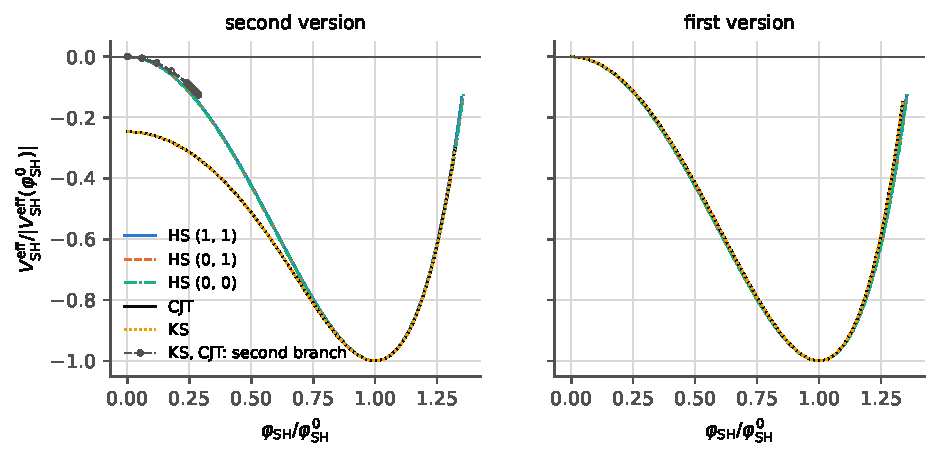
\includegraphics[width=0.9\textwidth]{figures/fig_sh_hg_potential.pdf}
\caption{\label{fig:potential}The effective potential divided by the depth of its minimum, against the pair amplitude,
for the five methods: the second version (left) and the first (right). KS and CJT coincide. The dashed line with circles
is the second branch of KS and CJT of the second version.}
\end{figure}

%=====================================================================================================================
\section{The susceptibilities and the masses of the gauge bosons}
\label{sec:gauge}

\subsection{Chemical potentials as the time components of the gauge fields}

A uniform, static gauge field couples to the charge densities. Its time component $A^a_0$ acts like a chemical potential
$\mu^a=g_aA^a_0$ of the charge $Q_a$. In the effective Lagrangian of the pair fields, $Z_\SH|D_\mu\Phi|^2$ gives for a
time component the term $Z_\SH\mu^2|Q\Phi|^2$, which lowers the energy of the superfluid by the same amount: the
susceptibilities
\begin{equation}
\chi^{ab}=\frac{\partial\langle Q_a\rangle}{\partial\mu^b}=-\frac{\partial^2\mathcal E}{\partial\mu^a\partial\mu^b}
\label{eq:chi}
\end{equation}
of the ground state of $H-\sum_b\mu^bQ_b$ are the coefficients of the mass term. The eight generators are $T^1$, $T^2$,
$T^3$, $T^1_R$, $T^2_R$, $T^3_R$, $R_\SH$ and $F^{\rm tot}_\SH$; the susceptibilities of the hypercharge
$Y=T^3_R+\tfrac14R_\SH$ are the corresponding combinations of theirs, and the mass matrix of $(W^1_\mu,W^2_\mu,W^3_\mu,B_\mu)$ is
\begin{equation}
(\mathsf M^{\rm g})^2_{ab}=g_ag_b\,\chi^{ab},\qquad a,b=1,2,3,Y,\qquad g_1=g_2=g_3=g,\quad g_Y=g',
\label{eq:Mg}
\end{equation}
where the index $a=1,2,3$ stands for $T^a$ and the index $Y$ for the hypercharge.
The space components of a uniform gauge field would also give it, but with the sharp cutoff of the momenta the normal
vacuum answers them with a current, an artifact that the time components avoid: the normal vacuum has a gap and does not
respond to a chemical potential at all. The program computes the ground states of $H-\mu^bQ_b$ for $\mu^b=\pm h$, $\pm2h$
($h=0.005$) and differentiates the charge densities $\langle Q_a\rangle=\tr(Q_a\varrho)$ by central differences with
Richardson extrapolation; by the theorem of Hellmann and Feynman $\partial\mathcal E/\partial\mu^a=-\langle Q_a\rangle$, so
$\chi$ must be symmetric. The Python program computes the same susceptibilities from the second derivatives of the
energy, a second method.

\subsection{Results}

Table~\ref{tab:chi} gives the susceptibilities. In every method they are symmetric, the row of $Q=T^3+Y$ vanishes (the
photon is massless), and the matrix of the eight generators has rank four in the second version; in the first, where of
$SU(2)_R$ only $T^3_R$ is a symmetry, the matrix of $T^1$, $T^2$, $T^3$, $R_\SH$ and $F^{\rm tot}_\SH$ has rank three. In
the second version the custodial structure $\chi(T^a)=\chi(T^a_R)=-\chi(T^a,T^a_R)$ holds, so $\chi^{YY}=\chi^{33}=-\chi^{3Y}$
and the mass matrix (\ref{eq:Mg}) has the eigenvalues $0$, $g^2\chi^{11}$ (twice) and $(g^2+g'^2)\chi^{33}$:
\begin{equation}
M_{W,\SH}=\tfrac12g\,v_\SH,\quad M_{Z,\SH}=\tfrac12(g^2+g'^2)^{1/2}v_\SH,\quad v_\SH=2(\chi^{11})^{1/2},\quad
\rho_\SH=\frac{\chi^{11}}{\chi^{33}}=1 .
\label{eq:rho}
\end{equation}
In the first version $\rho_\SH$ is \ensuremath{1.202}\mbox{--}\ensuremath{1.247}, which the measured $M_W^2/(M_Z^2\cos^2\hat\theta_W)=1.0103$ (with the
$\overline{\rm MS}$ angle $\sin^2\hat\theta_W(M_Z)=0.23122$~\cite{PDG2026}) excludes. Table~\ref{tab:scale} gives the scale
and the masses in GeV, with $v_\SH=v$, and Table~\ref{tab:gapgev} the gap in GeV: the lightest fermionic excitations, of
the charges $\frac34$ and $-\frac14$.

\begin{table}[!htbp]
\caption{\label{tab:chi}The susceptibilities ($10^3$ times their values) and $\rho_\SH$.}
\begingroup\centering\footnotesize\setlength{\tabcolsep}{4pt}
\begin{tabular}{llllllll}
\hline\hline
version & method & $\chi^{11}$ & $\chi^{33}$ & $\chi^{YY}$ & $\chi^{3Y}$ & $\chi^{FF}$ & $\rho_{\rm SH}$ \\ \hline
second & HS (1, 1) & $2.73681$ & $2.73681$ & $2.73681$ & $-2.73681$ & $43.4088$ & $1$ \\
second & HS (0, 1) & $2.60214$ & $2.60214$ & $2.60214$ & $-2.60214$ & $41.2905$ & $1$ \\
second & HS (0, 0) & $2.60214$ & $2.60214$ & $2.60214$ & $-2.60214$ & $41.6343$ & $1$ \\
second & KS & $3.11209$ & $3.11209$ & $3.11209$ & $-3.11209$ & $58.367$ & $1$ \\
second & CJT & $3.11209$ & $3.11209$ & $3.11209$ & $-3.11209$ & $58.367$ & $1$ \\
first & HS (1, 1) & $1.66832$ & $1.33798$ & $1.33798$ & $-1.33798$ & $21.4077$ & $1.2468945$ \\
first & HS (0, 1) & $1.59944$ & $1.29568$ & $1.29568$ & $-1.29568$ & $20.7308$ & $1.2344421$ \\
first & HS (0, 0) & $1.59944$ & $1.30107$ & $1.30107$ & $-1.30107$ & $20.8171$ & $1.2293239$ \\
first & KS & $1.88651$ & $1.56984$ & $1.56984$ & $-1.56984$ & $25.1174$ & $1.2017215$ \\
first & CJT & $1.88651$ & $1.56984$ & $1.56984$ & $-1.56984$ & $25.1174$ & $1.2017215$ \\
\hline\hline
\end{tabular}\par
\endgroup
\end{table}

\begin{table}[!htbp]
\caption{\label{tab:scale}The scale and the masses of the gauge bosons, with $v_\SH=246.22$ GeV.}
\begingroup\centering\footnotesize\setlength{\tabcolsep}{4pt}
\begin{tabular}{lllllll}
\hline\hline
version & method & $v_{\rm SH}$ (units of $\Lambda_{\rm LL}$) & $\Lambda_{\rm LL}$ (GeV) & $M_{W,{\rm SH}}$ (GeV) & $M_{Z,{\rm SH}}$ (GeV) & $\rho_{\rm SH}$ \\ \hline
second & HS (1, 1) & $0.104629$ & $2353.3$ & $80.3625$ & $91.1879$ & $1$ \\
second & HS (0, 1) & $0.102022$ & $2413.4$ & $80.3625$ & $91.1879$ & $1$ \\
second & HS (0, 0) & $0.102022$ & $2413.4$ & $80.3625$ & $91.1879$ & $1$ \\
second & KS & $0.111572$ & $2206.8$ & $80.3625$ & $91.1879$ & $1$ \\
second & CJT & $0.111572$ & $2206.8$ & $80.3625$ & $91.1879$ & $1$ \\
first & HS (1, 1) & $0.0816903$ & $3014.1$ & $80.3625$ & $81.6624$ & $1.24689$ \\
first & HS (0, 1) & $0.0799859$ & $3078.3$ & $80.3625$ & $82.0733$ & $1.23444$ \\
first & HS (0, 0) & $0.0799859$ & $3078.3$ & $80.3625$ & $82.244$ & $1.22932$ \\
first & KS & $0.0868678$ & $2834.4$ & $80.3625$ & $83.1831$ & $1.20172$ \\
first & CJT & $0.0868678$ & $2834.4$ & $80.3625$ & $83.1831$ & $1.20172$ \\
\hline\hline
\end{tabular}\par
\endgroup
\end{table}

\begin{table}[!htbp]
\caption{\label{tab:gapgev}The gap of the ground states in units of the cutoff and in GeV.}
\begingroup\centering\footnotesize\setlength{\tabcolsep}{4pt}
\begin{tabular}{llll}
\hline\hline
version & method & $E^{X,{\rm gap}}$ (units of $\Lambda_{\rm LL}$) & $E^{X,{\rm gap}}$ (GeV) \\ \hline
second & HS (1, 1) & $0.426792$ & $1004.4$ \\
second & HS (0, 1) & $0.452967$ & $1093.2$ \\
second & HS (0, 0) & $0.452967$ & $1093.2$ \\
second & KS & $0.384201$ & $847.86$ \\
second & CJT & $0.384201$ & $847.86$ \\
first & HS (1, 1) & $0.170392$ & $513.57$ \\
first & HS (0, 1) & $0.2$ & $615.66$ \\
first & HS (0, 0) & $0.2$ & $615.66$ \\
first & KS & $0.111459$ & $315.92$ \\
first & CJT & $0.111459$ & $315.92$ \\
\hline\hline
\end{tabular}\par
\endgroup
\end{table}

%=====================================================================================================================
\section{The amplitude mode}
\label{sec:amplitude}

\subsection{The effective Lagrangian}

At long wavelengths the pair fields obey $Z_\SH(|\partial\Phi^{\rm d}|^2+|\partial\Phi'^{\rm u}|^2)-V^{\rm eff}_\SH$ (second
version). A chemical potential $\mu$ of $T^3$, under which $\Phi^{\rm d}$ has the charge $-\frac12$ and $\Phi'^{\rm u}$ the
charge $+\frac12$, lowers the energy by $Z_\SH\mu^2(\frac14+\frac14)(\varphi^0_\SH)^2$, so $\chi^{33}=Z_\SH(\varphi^0_\SH)^2$.
When both lengths oscillate together, $\varphi_\SH=\varphi^0_\SH+\eta$, the kinetic term is $2Z_\SH\dot\eta^2$ and the potential
$\frac12V^{\rm eff\,\prime\prime}_\SH\eta^2$, so
\begin{equation}
(M^{\rm EFT}_\SH)^2=\frac{V^{\rm eff\,\prime\prime}_\SH(\varphi^0_\SH)\,(\varphi^0_\SH)^2}{4\chi^{33}} .
\label{eq:MEFT}
\end{equation}
The same formula holds in the first version, with $\chi^{33}=\frac12Z_\SH(\varphi^0_\SH)^2$ and the kinetic term
$Z_\SH\dot\eta^2$. Formula (\ref{eq:MEFT}) is the leading order of an expansion in the frequency; Table~\ref{tab:amp} shows that
the mode lies close to the energy $2E^{X,{\rm gap}}$ that breaks a pair, where that expansion fails.

\begin{table}[!htbp]
\caption{\label{tab:amp}The amplitude mode from the effective Lagrangian, and twice the gap, the lowest energy of two quasi-particles.}
\begingroup\centering\footnotesize\setlength{\tabcolsep}{4pt}
\begin{tabular}{llllll}
\hline\hline
version & method & $M^{\rm EFT}_{\rm SH}$ & $M^{\rm EFT}_{\rm SH}/v_{\rm SH}$ & $M^{\rm EFT}_{\rm SH}$ (GeV) & $2E^{X,{\rm gap}}$ \\ \hline
second & HS (1, 1) & $0.96457$ & $9.219$ & $2270$ & $0.85358$ \\
second & HS (0, 1) & $0.94638$ & $9.276$ & $2284$ & $0.90593$ \\
second & HS (0, 0) & $0.94638$ & $9.276$ & $2284$ & $0.90593$ \\
second & KS & $1.0676$ & $9.569$ & $2356$ & $0.7684$ \\
second & CJT & $1.0676$ & $9.569$ & $2356$ & $0.7684$ \\
first & HS (1, 1) & $0.95778$ & $11.72$ & $2887$ & $0.34078$ \\
first & HS (0, 1) & $0.94835$ & $11.86$ & $2919$ & $0.4$ \\
first & HS (0, 0) & $0.94638$ & $11.83$ & $2913$ & $0.4$ \\
first & KS & $0.97123$ & $11.18$ & $2753$ & $0.22292$ \\
first & CJT & $0.97123$ & $11.18$ & $2753$ & $0.22292$ \\
\hline\hline
\end{tabular}\par
\endgroup
\end{table}

\subsection{The linear response}

A uniform fluctuation with the time factor $e^{-i\omega t}$ changes the self-energies by complex amplitudes $\delta\mathsf N$,
$\delta\mathsf P$ and $\delta\bar{\mathsf P}$ (independent at a real frequency). In the eigenbasis $(E_k,|k\rangle)$ of
(\ref{eq:BdG}) at each momentum the change of the projector onto the negative eigenvalues is
\begin{equation}
\delta R_{kl}=\delta H_{kl}\,\frac{f_l-f_k}{\omega-E_k+E_l},\qquad f_k=1\ \text{for}\ E_k<0,\ 0\ \text{otherwise},
\label{eq:dR}
\end{equation}
summed over the momenta; this is the response $\bm\chi(\omega)$ of the local matrices. The contact terms map the changes of
the local matrices back to the self-energies by the kernel $\mathsf F^X$, and a collective mode is a frequency at which
$1-\bm\chi(\omega)\mathsf F^X$ is singular. The program computes it in the sector of relative number 0 (the normal blocks of
$\Psi_\LL$ and of the pair of singlets and the pairs of $\Psi_\LL$ with the singlets, closed under the symmetries of the
state), in HS (0,1) and HS (0,0), where the mode lies below the threshold $2M_{\rm eff}$ of two paired quasi-particles. It
searches the frequencies below the threshold for zeros of the smallest singular value, finds the null space at each zero,
and projects onto it the amplitude of the vacuum direction; the amplitude mode is the zero whose null space contains it,
and the dimension of the null space is its multiplicity. Table~\ref{tab:rpa} gives the results: at $\omega=0$ exactly
four singular values vanish in the second version (three in the first), the Goldstone modes, and below the threshold the
amplitude mode lies at $\omega^{\rm H}_\SH=d^0_\SH$ to \ensuremath{2\times10^{-13}}.

\begin{table}[!htbp]
\caption{\label{tab:rpa}The amplitude mode from the linear response in the pairing-only methods: its frequency, its departure from $d^0_\SH$, the ratio to the scale, the frequency in GeV, the lowest transition energy whose terms act on its null space, and its multiplicity.}
\begingroup\centering\footnotesize\setlength{\tabcolsep}{4pt}
\begin{tabular}{llcccccc}
\hline\hline
version & method & $\omega^{\rm H}_{\rm SH}$ & $\omega^{\rm H}_{\rm SH}/d^0_{\rm SH}-1$ & $\omega^{\rm H}_{\rm SH}/v_{\rm SH}$ & $\omega^{\rm H}_{\rm SH}$ (GeV) & lowest transition that acts on it & multiplicity \\ \hline
second & HS (0, 1) & $0.8128455463$ & $-2\times10^{-13}$ & $7.967$ & $1962$ & $0.905948$ & 4 \\
second & HS (0, 0) & $0.8128455463$ & $-2\times10^{-13}$ & $7.967$ & $1962$ & $0.905948$ & 4 \\
first & HS (0, 1) & $0.8128455463$ & $-2\times10^{-13}$ & $10.16$ & $2502$ & $0.905948$ & 1 \\
first & HS (0, 0) & $0.8128455463$ & $-2\times10^{-13}$ & $10.16$ & $2502$ & $0.905948$ & 1 \\
\hline\hline
\end{tabular}\par
\endgroup
\end{table}

\subsection{The closed form of the pairing-only methods}

In HS (0,0) the response of the pair amplitudes takes the form of the theory of Bardeen, Cooper and
Schrieffer~\cite{BCS1957}. With $E=(q^2+M_{\rm eff}^2)^{1/2}$ the eigenvalues along the amplitude and along the phase of the
vacuum direction are
\begin{equation}
\lambda^{\rm amp}(\omega)=\frac{G_\SH}{4\pi^2}\int_0^{\Lambda_\LL}\frac{q^2(q^2+m_\LL^2)\,dq}{E\,(E^2-\omega^2/4)},\qquad
\lambda^{\rm ph}(\omega)=\frac{G_\SH}{4\pi^2}\int_0^{\Lambda_\LL}\frac{q^2E\,dq}{E^2-\omega^2/4},
\label{eq:lam}
\end{equation}
as sums over the nodes of the grid with its weights. The Python program finds that its response equals these sums to
\ensuremath{10^{-15}} at five frequencies, in both versions. At $\omega=0$, $\lambda^{\rm ph}(0)=G_\SH I_1(M_{\rm eff})/(4\pi^2)=1$ is the
gap equation and the Goldstone theorem. Since $E^2=q^2+m_\LL^2+(d^0_\SH)^2/4$, the integrands obey, at every momentum,
\begin{equation}
\frac{q^2+m_\LL^2}{E\,(E^2-\omega^2/4)}-\frac1E=\frac{\omega^2-(d^0_\SH)^2}{4E\,(E^2-\omega^2/4)},
\end{equation}
and with the gap equation
\begin{equation}
\lambda^{\rm amp}(\omega)-1=\frac{\omega^2-(d^0_\SH)^2}{4}\,\frac{G_\SH}{4\pi^2}\int_0^{\Lambda_\LL}\frac{q^2\,dq}{E\,(E^2-\omega^2/4)} .
\label{eq:identity}
\end{equation}
Below the threshold every term of the integral is positive, so $\lambda^{\rm amp}=1$ only at
\begin{equation}
\omega^{\rm H}_\SH=d^0_\SH ,
\label{eq:omegaH}
\end{equation}
exactly, for every coupling, mass and cutoff and on every grid with positive weights. The mode is bound by
$2M_{\rm eff}-d^0_\SH=(4m_\LL^2+(d^0_\SH)^2)^{1/2}-d^0_\SH=0.09309$. The Wolfram script derives (\ref{eq:identity}) and the
positivity symbolically and finds the root at $d^0_\SH$ to 22 digits. Result (\ref{eq:omegaH}) is the analogue of the
amplitude mode of a superconductor at twice the gap parameter~\cite{LittlewoodVarma1981,PekkerVarma2015}; here $d^0_\SH/2$
plays the role of the gap parameter, and the mass of the fields raises the lowest energy of a quasi-particle from
$d^0_\SH/2$ to $M_{\rm eff}$, so that the mode is bound.

\emph{The partners of the amplitude mode.} On the eight real components of the four complex pair fields the Python
program finds four eigenvalues equal to 1 at $\omega=0$ and four more at $\omega=d^0_\SH$. The generators $T^a+T^a_R$ of
$SU(2)_V$ commute with the response, and on each set the Casimir $\sum_a(T^a+T^a_R)^2$ has the eigenvalues 0, 2, 2, 2: a
singlet and a triplet. At $\omega=0$ the triplet becomes the longitudinal parts of $W^\pm_\mu$ and $Z_\mu$ and the singlet is
the Goldstone boson of $F^{\rm tot}_\SH$; at $\omega=d^0_\SH$ the singlet is the amplitude mode, and the triplet holds a
neutral scalar and a charged scalar with its antiparticle ($Q=T^3+T^3_R$ on the pair fields). In the first version the
same count gives three Goldstone modes and one amplitude mode, as in the Standard Model.

\subsection{The dependence on the coupling and the mass}

In HS (0,0) the gap equation $G_\SH I_1(M_{\rm eff})/(4\pi^2)=1$ gives $d^0_\SH$ in closed form, so the amplitude mode and the
scale can be followed over the coupling. Table~\ref{tab:scan} gives 32 points: $m_\LL=0.1$ and $0.2$,
$G_\SH/G^{\rm crit}_\SH$ from 1.02 to 3, both versions. In every point the Rust program finds the self-consistent state, the
amplitude mode at $d^0_\SH$ to \ensuremath{2\times10^{-12}}, and $\rho_\SH=1$ in the second version; $\omega^{\rm H}_\SH/v_\SH$ lies between
\ensuremath{4.892} and \ensuremath{34.43} in the second version, against $m_H/v=0.5082$.

\begin{table}[!htbp]
\caption{\label{tab:scan}The scan of HS (0,0): the mass, the coupling, the pair self-energy, the scale, $\rho_\SH$, the amplitude mode, the threshold and the ratio of the mode to the scale.}
\begingroup\centering\footnotesize\setlength{\tabcolsep}{4pt}
\begin{tabular}{lllllllll}
\hline\hline
version & $m_{\rm LL}$ & $G_{\rm SH}/G^{\rm crit}_{\rm SH}$ & $d^0_{\rm SH}$ & $v_{\rm SH}$ & $\rho_{\rm SH}$ & $\omega^{\rm H}_{\rm SH}$ & $2M_{\rm eff}$ & $\omega^{\rm H}_{\rm SH}/v_{\rm SH}$ \\ \hline
second & $0.1$ & $1.02$ & $0.20583$ & $0.042078$ & $1$ & $0.205833$ & $0.286997$ & $4.892$ \\
second & $0.1$ & $1.05$ & $0.34088$ & $0.062877$ & $1$ & $0.340883$ & $0.395223$ & $5.421$ \\
second & $0.1$ & $1.1$ & $0.50977$ & $0.082828$ & $1$ & $0.509767$ & $0.547597$ & $6.155$ \\
second & $0.1$ & $1.1838$ & $0.73828$ & $0.1021$ & $1$ & $0.738278$ & $0.764889$ & $7.231$ \\
second & $0.1$ & $1.3$ & $1.0064$ & $0.11671$ & $1$ & $1.00635$ & $1.02604$ & $8.623$ \\
second & $0.1$ & $1.5$ & $1.4071$ & $0.12807$ & $1$ & $1.40709$ & $1.42123$ & $10.99$ \\
second & $0.1$ & $2$ & $2.2705$ & $0.13152$ & $1$ & $2.2705$ & $2.2793$ & $17.26$ \\
second & $0.1$ & $3$ & $3.8001$ & $0.11903$ & $1$ & $3.80008$ & $3.80534$ & $31.92$ \\
second & $0.2$ & $1.02$ & $0.24066$ & $0.041741$ & $1$ & $0.240656$ & $0.466814$ & $5.765$ \\
second & $0.2$ & $1.05$ & $0.39029$ & $0.062858$ & $1$ & $0.390293$ & $0.558864$ & $6.209$ \\
second & $0.2$ & $1.1$ & $0.57181$ & $0.082962$ & $1$ & $0.571812$ & $0.697832$ & $6.892$ \\
second & $0.2$ & $1.1838$ & $0.81285$ & $0.10202$ & $1$ & $0.812846$ & $0.905935$ & $7.967$ \\
second & $0.2$ & $1.3$ & $1.0931$ & $0.11615$ & $1$ & $1.09305$ & $1.16394$ & $9.411$ \\
second & $0.2$ & $1.5$ & $1.5106$ & $0.12679$ & $1$ & $1.51061$ & $1.56267$ & $11.91$ \\
second & $0.2$ & $2$ & $2.411$ & $0.12934$ & $1$ & $2.41104$ & $2.444$ & $18.64$ \\
second & $0.2$ & $3$ & $4.0115$ & $0.11652$ & $1$ & $4.01146$ & $4.03136$ & $34.43$ \\
first & $0.1$ & $1.02$ & $0.20583$ & $0.030618$ & $1.05896$ & $0.205833$ & $0.286997$ & $6.723$ \\
first & $0.1$ & $1.05$ & $0.34088$ & $0.046903$ & $1.11287$ & $0.340883$ & $0.395223$ & $7.268$ \\
first & $0.1$ & $1.1$ & $0.50977$ & $0.06347$ & $1.1744$ & $0.509767$ & $0.547597$ & $8.032$ \\
first & $0.1$ & $1.1838$ & $0.73828$ & $0.080797$ & $1.25253$ & $0.738278$ & $0.764889$ & $9.137$ \\
first & $0.1$ & $1.3$ & $1.0064$ & $0.095641$ & $1.34313$ & $1.00635$ & $1.02604$ & $10.52$ \\
first & $0.1$ & $1.5$ & $1.4071$ & $0.11017$ & $1.48008$ & $1.40709$ & $1.42123$ & $12.77$ \\
first & $0.1$ & $2$ & $2.2705$ & $0.12369$ & $1.76891$ & $2.2705$ & $2.2793$ & $18.36$ \\
first & $0.1$ & $3$ & $3.8001$ & $0.12476$ & $2.19689$ & $3.80008$ & $3.80534$ & $30.46$ \\
first & $0.2$ & $1.02$ & $0.24066$ & $0.030059$ & $1.03721$ & $0.240656$ & $0.466814$ & $8.006$ \\
first & $0.2$ & $1.05$ & $0.39029$ & $0.046256$ & $1.08303$ & $0.390293$ & $0.558864$ & $8.438$ \\
first & $0.2$ & $1.1$ & $0.57181$ & $0.062771$ & $1.14496$ & $0.571812$ & $0.697832$ & $9.109$ \\
first & $0.2$ & $1.1838$ & $0.81285$ & $0.079986$ & $1.22932$ & $0.812846$ & $0.905935$ & $10.16$ \\
first & $0.2$ & $1.3$ & $1.0931$ & $0.09464$ & $1.32786$ & $1.09305$ & $1.16394$ & $11.55$ \\
first & $0.2$ & $1.5$ & $1.5106$ & $0.10886$ & $1.47434$ & $1.51061$ & $1.56267$ & $13.88$ \\
first & $0.2$ & $2$ & $2.411$ & $0.12187$ & $1.77559$ & $2.41104$ & $2.444$ & $19.78$ \\
first & $0.2$ & $3$ & $4.0115$ & $0.12254$ & $2.21203$ & $4.01146$ & $4.03136$ & $32.74$ \\
\hline\hline
\end{tabular}\par
\endgroup
\end{table}

%=====================================================================================================================
\section{The dynamics in time}
\label{sec:dynamics}

The time-dependent mean field of method $X$ evolves the quasi-particle vectors of every momentum by the BdG matrix of the
self-energies that the current local matrices produce,
\begin{equation}
i\,\partial_t\,\mathsf O(\vec q,t)=\mathsf H(\vec q;\mathsf N(t),\mathsf P(t))\,\mathsf O(\vec q,t),
\label{eq:tdmf}
\end{equation}
whose linearization about a stationary state is the linear response (\ref{eq:dR}). The program integrates it with the
backward differentiation formulas of CVODE~\cite{SUNDIALS2005,SUNDIALS2022} (relative tolerance $10^{-12}$, absolute
$10^{-14}$, the Newton iteration replaced by a fixed-point iteration), on the same grid as the stationary states. A run
starts from the ground state with the pair self-energy displaced by the relative amount $\epsilon^{\rm kick}$ along the
vacuum direction (an amplitude run) or along the custodial triplet (a triplet run), and records $d(t)$; its spectrum is
the Fourier transform over the run, with the peak frequency $\omega^{\rm pk}$ and the half-width $\Gamma^{\rm pk}$, compared
with the half-width $\Gamma^{\rm win}$ that the length of the run alone gives. Table~\ref{tab:runs} lists the runs with the
conservation of the energy, of the charges and of the orthonormality of the vectors, and Table~\ref{tab:modes} the modes.

\begin{table}[!htbp]
\caption{\label{tab:runs}The runs in time: the kind, the version, the method, the displacement, the largest relative changes of the energy and of the charges and the departure from orthonormality, the steps of CVODE, and the computing time.}
\begingroup\centering\footnotesize\setlength{\tabcolsep}{4pt}
\begin{tabular}{lllllllll}
\hline\hline
run & version & method & $\epsilon^{\rm kick}$ & energy & charges & $\mathsf O^\dagger\mathsf O-\mathsf 1$ & steps & time (s) \\ \hline
amplitude & second & HS (1, 1) & $0.001$ & $5\times10^{-7}$ & $5\times10^{-10}$ & $2\times10^{-8}$ & 6092 & 157 \\
triplet & second & HS (1, 1) & $0.001$ & $6\times10^{-8}$ & $6\times10^{-11}$ & $2\times10^{-9}$ & 7971 & 125 \\
amplitude & second & HS (0, 1) & $0.001$ & $9\times10^{-8}$ & $10^{-10}$ & $3\times10^{-9}$ & 7458 & 127 \\
triplet & second & HS (0, 1) & $0.001$ & $3\times10^{-7}$ & $3\times10^{-10}$ & $6\times10^{-9}$ & 6524 & 130 \\
ground & second & HS (0, 0) & -- & $6\times10^{-8}$ & $7\times10^{-11}$ & $2\times10^{-9}$ & 2280 & 45 \\
josephson & second & HS (0, 0) & -- & $7\times10^{-8}$ & $7\times10^{-11}$ & $2\times10^{-9}$ & 2281 & 47 \\
amplitude & second & HS (0, 0) & $0.001$ & $5\times10^{-7}$ & $5\times10^{-10}$ & $2\times10^{-8}$ & 6104 & 140 \\
triplet & second & HS (0, 0) & $0.001$ & $6\times10^{-8}$ & $6\times10^{-11}$ & $2\times10^{-9}$ & 8087 & 138 \\
large & second & HS (0, 0) & $0.3$ & $2\times10^{-8}$ & $2\times10^{-11}$ & $4\times10^{-10}$ & 9703 & 155 \\
amplitude & second & KS & $0.001$ & $3\times10^{-8}$ & $5\times10^{-11}$ & $2\times10^{-9}$ & 8349 & 153 \\
triplet & second & KS & $0.001$ & $4\times10^{-8}$ & $6\times10^{-11}$ & $2\times10^{-9}$ & 8122 & 143 \\
ground & second & CJT & -- & $9\times10^{-9}$ & $2\times10^{-11}$ & $4\times10^{-10}$ & 2800 & 43 \\
josephson & second & CJT & -- & $9\times10^{-9}$ & $2\times10^{-11}$ & $4\times10^{-10}$ & 2807 & 43 \\
amplitude & second & CJT & $0.001$ & $3\times10^{-8}$ & $5\times10^{-11}$ & $2\times10^{-9}$ & 8350 & 128 \\
triplet & second & CJT & $0.001$ & $2\times10^{-7}$ & $3\times10^{-10}$ & $7\times10^{-9}$ & 6532 & 114 \\
amplitude & first & HS (1, 1) & $0.001$ & $10^{-6}$ & $6\times10^{-10}$ & $2\times10^{-8}$ & 5695 & 119 \\
amplitude & first & HS (0, 1) & $0.001$ & $2\times10^{-6}$ & $6\times10^{-10}$ & $2\times10^{-8}$ & 5639 & 131 \\
amplitude & first & HS (0, 0) & $0.001$ & $2\times10^{-6}$ & $6\times10^{-10}$ & $2\times10^{-8}$ & 5694 & 129 \\
large & first & HS (0, 0) & $0.3$ & $6\times10^{-8}$ & $3\times10^{-11}$ & $9\times10^{-10}$ & 8657 & 142 \\
amplitude & first & KS & $0.001$ & $9\times10^{-7}$ & $6\times10^{-10}$ & $2\times10^{-8}$ & 5721 & 136 \\
amplitude & first & CJT & $0.001$ & $10^{-6}$ & $7\times10^{-10}$ & $2\times10^{-8}$ & 5601 & 121 \\
\hline\hline
\end{tabular}\par
\endgroup
\end{table}

\begin{table}[!htbp]
\caption{\label{tab:modes}The modes in time: $d^0_\SH$, twice the gap, and the peak and the ratio of its half-width to that of the window, for the amplitude and the triplet runs.}
\begingroup\centering\footnotesize\setlength{\tabcolsep}{4pt}
\begin{tabular}{llllllll}
\hline\hline
version & method & $d^0_{\rm SH}$ & $2E^{X,{\rm gap}}$ & $\omega^{\rm pk}$, amplitude & $\Gamma^{\rm pk}/\Gamma^{\rm win}$ & $\omega^{\rm pk}$, triplet & $\Gamma^{\rm pk}/\Gamma^{\rm win}$ \\ \hline
second & HS (1, 1) & $0.8328776$ & $0.853584$ & $0.8108707$ & $1$ & $0.8285249$ & $1$ \\
second & HS (0, 1) & $0.8128455$ & $0.905935$ & $0.8128465$ & $1$ & $0.8128465$ & $1$ \\
second & HS (0, 0) & $0.8128455$ & $0.905935$ & $0.8128465$ & $1$ & $0.8128465$ & $1$ \\
second & KS & $0.8907872$ & $0.768402$ & $0.8735459$ & $1.8$ & $0.8687108$ & $2.12$ \\
second & CJT & $0.8907872$ & $0.768402$ & $0.8735459$ & $1.8$ & $0.8687108$ & $2.12$ \\
first & HS (1, 1) & $0.8258096$ & $0.340784$ & $0.8061557$ & $1.04$ & -- & -- \\
first & HS (0, 1) & $0.8128455$ & $0.4$ & $0.8128466$ & $1$ & -- & -- \\
first & HS (0, 0) & $0.8128455$ & $0.4$ & $0.8128466$ & $1$ & -- & -- \\
first & KS & $0.8672856$ & $0.222918$ & $0.8525918$ & $2.16$ & -- & -- \\
first & CJT & $0.8672856$ & $0.222918$ & $0.8525918$ & $2.16$ & -- & -- \\
\hline\hline
\end{tabular}\par
\endgroup
\end{table}

In HS (0,1) and HS (0,0) the amplitude run oscillates at $d^0_\SH$ to \ensuremath{2\times10^{-6}}, without damping, and the triplet run
at the same frequency. In HS (1,1) the mode lies at 0.9736\,$d^0_\SH$, below $2E^{X,{\rm gap}}$, undamped, and the
triplet 2.2 per cent above it. In KS and CJT the spectrum peaks at 0.873546, above $2E^{X,{\rm gap}}=0.768402$,
1.8 times wider than an undamped oscillation: the mode decays into pairs. With a chemical potential $\mu=0.01$ of
the particle number the phase turns at the rate $2\mu$ to \ensuremath{2\times10^{-9}} (the Josephson relation), and a displacement by
$\epsilon^{\rm kick}=0.3$ in HS (0,0) oscillates at 0.9582\,$d^0_\SH$, softer than the small oscillation.

%=====================================================================================================================
\section{Toward the gravitational sector: Lord's construction}
\label{sec:gravity}

Lord~\cite{Lord1971} considered the group of the local changes of representation of the two-component spinor algebra,
under which the free field equations of particles of any spin are invariant, and made it a gauge group in the sense of
Yang and Mills. Gauge invariance and Lorentz covariance then require auxiliary fields, which Lord interpreted as the
potentials of a spin-two field; that field is self-interacting, and the Bargmann-Wigner equations of the linear spin-two
field, modified by the self-interaction, give a nonlinear theory identical with Einstein's, the auxiliary fields becoming
in addition the gauge field of the general coordinate transformations. In the present model the factor $SL(2,\mathbb C)$
of the gauge group acts on the spinor indices of the three fields with the connection $\Gamma^\LL_\mu$ of (\ref{eq:cov}),
a pure gauge on flat space-time. The program is to replace $\Gamma^\LL_\mu$ by Lord's gauge field and its auxiliary fields,
to couple the spinor fields and their pairs to it, and to obtain the gravitational field equations with the
energy-momentum tensor of the spinor fields as their source; the route of Utiyama and Kibble~\cite{Utiyama1956,Kibble1961,Hehl1976}
gauges the local Lorentz group in the same spirit. None of this is computed here.

%=====================================================================================================================
\section{The checks}
\label{sec:checks}

The computation was made in stages, each with a program in Rust, one in Python and a script in the Wolfram Language:
stage 2, the group theory and the quantum numbers (sh\_quantum, Sec.~\ref{sec:model}); stage 3, the normal vacuum and the
stationary states (sh\_superfluid, Secs.~\ref{sec:methods} to \ref{sec:states}); stages 4 and 5, the effective potential,
the masses of the gauge bosons and the amplitude mode (sh\_higgs, Secs.~\ref{sec:potential} to \ref{sec:amplitude}); and
stage 6, the dynamics in time (sh\_dynamics, Sec.~\ref{sec:dynamics}). Stage 1 set out the hypotheses.
Every statement of the article and of this Supplemental Material is tested by checks of the programs; each check
compares a computed deviation with a tolerance, or decides a statement that is true or false from the facts that the
program states. The statements of the checks are those that the programs write; where they cite the hypotheses or the
equations of the manuscripts of the stages, the tables below cite instead the place of this Supplemental Material that
states the same thing. The verdicts: the Rust programs stage 2 (\texttt{sh\_quantum}) ALL PASS (55 of 55); stage 3 (\texttt{sh\_superfluid}) ALL PASS (25 of 25); stage 4 (\texttt{sh\_higgs}) ALL PASS (30 of 30); stage 6 (\texttt{sh\_dynamics}) ALL PASS (12 of 12); the Python programs stage 2 ALL PASS (14 of 14); stage 3 ALL PASS (8 of 8); stage 4 ALL PASS (10 of 10); stage 6 ALL PASS (7 of 7); the Wolfram
scripts stage 2 ALL PASS (13 of 13); stage 3 ALL PASS (5 of 5); stage 4 ALL PASS (5 of 5); stage 6 ALL PASS (5 of 5); the notebook, which repeats the checks of the Wolfram scripts, ALL PASS (181 of 181), 0 messages; its Part R repeats the 28 checks of the Wolfram scripts of the revision, and 28 of them pass. The
worked examples of Sec.~II of the article (the octonions, the Lorentz super-loop, the spinor charges, the spinors and
isodoublets, and the superfluid of the spinor charges) are computed by a further Rust program, \texttt{rust/shexamples},
recomputed by \texttt{python/sh\_examples.py} and derived symbolically by \texttt{wolfram/source/sh\_examples.wls}; their
verdicts: Rust ALL PASS (27 of 27); Python ALL PASS (9 of 9); Wolfram ALL PASS (6 of 6). The tables list every check of the Rust and the Python programs of the stages with its
result, deviation, tolerance and statement.

\begingroup\fontsize{7}{8.5}\selectfont\setlength{\tabcolsep}{3pt}
\begin{longtable}{p{0.09\textwidth}p{0.05\textwidth}p{0.085\textwidth}p{0.075\textwidth}p{0.64\textwidth}}
\caption{\label{tab:checks_quantum_rust}The checks of the Rust program of stage 2 (\texttt{data/hck\_sh\_quantum\_checks.txt}).}\\
\hline\hline
check & result & deviation & tolerance & statement \\ \hline
\endfirsthead
\hline check & result & deviation & tolerance & statement \\ \hline
\endhead
\hline\hline
\endlastfoot
QN-1a & PASS & 0.000e0 & 1.0e-12 & [T\textasciicircum{}a, T\textasciicircum{}b] = i eps\_abc T\textasciicircum{}c on the sixteen components (the algebra of SU(2)\_L) \\
QN-1b & PASS & 0.000e0 & 1.0e-12 & [T\textasciicircum{}a\_R, T\textasciicircum{}b\_R] = i eps\_abc T\textasciicircum{}c\_R (the algebra of the custodial SU(2)\_R) and [T\textasciicircum{}a, T\textasciicircum{}b\_R] = 0 \\
QN-1c & PASS & 0.000e0 & 1.0e-12 & Y, F\_tot, R and T\textasciicircum{}3\_R commute with T\textasciicircum{}1, T\textasciicircum{}2, T\textasciicircum{}3 and with each other, and F\_tot and R commute with T\textasciicircum{}a\_R (the global group SU(2)\_L x SU(2)\_R x U(1)\_R x U(1)\_F\_tot of Sec.~\ref{sec:model}) \\
QN-1d & PASS & 0.000e0 & 1.0e-12 & T\textasciicircum{}a, T\textasciicircum{}a\_R, Y, Q, F\_tot, R are Hermitian (a unitary representation) \\
QN-1e & PASS & -- & -- & Y = T\textasciicircum{}3\_R + R/4 (equation (\ref{eq:Y})) and Q = T\textasciicircum{}3 + T\textasciicircum{}3\_R + R/4; Y does not commute with T\textasciicircum{}1\_R (the coupling of B to Y breaks SU(2)\_R to the U(1) of T\textasciicircum{}3\_R) [deviations 0.0e0 and 0.0e0; largest entry of [Y, T\textasciicircum{}1\_R] 1/2] \\
QN-2a & PASS & -- & -- & the six real generators S(u) = diag(-M(u)\textasciicircum{}dag, M(u)) on each field satisfy S([u, u']) = [S(u), S(u')] and are independent over the real numbers [largest deviation 0.0e0; smallest eigenvalue of the real Gram matrix 4.0000] \\
QN-2b & PASS & 0.000e0 & 1.0e-12 & the Lorentz generators commute with T\textasciicircum{}a, T\textasciicircum{}a\_R, Y, Q, F\_tot, R (space-time and internal symmetries) \\
QN-3a & PASS & 0.000e0 & 1.0e-12 & the free Hamiltonian diag(h\_Psi(q), h\_chi(q), h\_chi'(q)) commutes with T\textasciicircum{}a, Y, Q, F\_tot, R, T\textasciicircum{}3\_R (25 random momenta; the masses m\_LL = 0.2, m\textasciicircum{}chi\_SH = 0.35, m\textasciicircum{}chi'\_SH = 0.5, or all three 0.2) \\
QN-3b & PASS & 0.000e0 & 1.0e-12 & with equal masses of the two singlets (m\textasciicircum{}chi\_SH = m\textasciicircum{}chi'\_SH = 0.35, m\_LL = 0.2) it commutes also with T\textasciicircum{}1\_R, T\textasciicircum{}2\_R, T\textasciicircum{}3\_R: SU(2)\_R is a symmetry of the free Lagrangian \\
QN-3c & PASS & 0.000e0 & 1.0e-12 & with unequal masses of the singlets (0.35 and 0.5) the largest entry of [h, T\textasciicircum{}1\_R] is \textbar{}m\textasciicircum{}chi\_SH - m\textasciicircum{}chi'\_SH\textbar{}/2: the difference of the masses breaks SU(2)\_R (deviation from that value) \\
QN-4a & PASS & 0.000e0 & 1.0e-12 & Y = 1/4 on Psi\_LL and chi\_SH and -3/4 on chi'\_SH; F\_LL = 4 Y equals F\_tot on Psi\_LL and chi\_SH (Sec.~\ref{sec:model}) and -3 F\_tot on chi'\_SH \\
QN-4b & PASS & 0.000e0 & 1.0e-12 & Q = T\textasciicircum{}3 + Y is 3/4 on the up components of Psi\_LL, -1/4 on the down components, 1/4 on chi\_SH and -3/4 on chi'\_SH \\
QN-4c & PASS & 0.000e0 & 1.0e-12 & the Casimir operators: sum\_a (T\textasciicircum{}a)\textasciicircum{}2 = 3/4 on Psi\_LL and 0 on the singlets, sum\_a (T\textasciicircum{}a\_R)\textasciicircum{}2 = 0 on Psi\_LL and 3/4 on chi\_SH and chi'\_SH (the pair of singlets is a doublet of SU(2)\_R) \\
QN-5a & PASS & 0.000e0 & 1.0e-12 & the anomaly traces tr(gamma\textasciicircum{}ch Y\textasciicircum{}3), tr(gamma\textasciicircum{}ch Y), tr(gamma\textasciicircum{}ch \{T\textasciicircum{}a, T\textasciicircum{}b\} Y), tr(gamma\textasciicircum{}ch Y\textasciicircum{}2 T\textasciicircum{}a), tr(gamma\textasciicircum{}ch T\textasciicircum{}a \{T\textasciicircum{}b, T\textasciicircum{}c\}) vanish (47 traces) \\
QN-5b & PASS & 0.000e0 & 1.0e-12 & the fields are vector-like: gamma\textasciicircum{}0, which exchanges the two chiralities, commutes with every internal generator \\
QN-5c & PASS & -- & -- & the number of Weyl doublets of SU(2)\_L is even (no global anomaly; the right-handed doublet counts as the conjugate of a left-handed one) [8 components with Casimir 3/4, 2 Weyl doublets] \\
QN-6a & PASS & -- & -- & the Lorentz-invariant pairs of the six sectors: dimensions 6 (Psi Psi, antisymmetric by Fermi statistics), 4 (Psi chi), 4 (Psi chi'), 2 (chi chi, antisymmetric), 2 (chi chi'), 2 (chi' chi', antisymmetric) [Psi Psi 6, Psi chi 4, Psi chi' 4, chi chi 2, chi chi' 2, chi' chi' 2; eigenvalues counted as zero at most 6.6e-15, the others at least 3.000] \\
QN-6b & PASS & -- & -- & the Lorentz-invariant particle-antiparticle bilinears of the six sectors: dimensions 8 (Psi\textasciicircum{}dag Psi), 4 (Psi\textasciicircum{}dag chi), 4 (Psi\textasciicircum{}dag chi'), 2 (chi\textasciicircum{}dag chi), 2 (chi\textasciicircum{}dag chi'), 2 (chi'\textasciicircum{}dag chi') [Psi\textasciicircum{}dag Psi 8, Psi\textasciicircum{}dag chi 4, Psi\textasciicircum{}dag chi' 4, chi\textasciicircum{}dag chi 2, chi\textasciicircum{}dag chi' 2, chi'\textasciicircum{}dag chi' 2; eigenvalues counted as zero at most 7.8e-16, the others at least 3.000] \\
QN-6c & PASS & -- & -- & the symmetric Lorentz-invariant matrices of two particles of one field, which give no operator (Fermi statistics): dimension 2 for Psi Psi, 0 for chi chi and chi' chi' [dimensions 2, 0, 0; gap 2.0e-15 / 3.000] \\
QN-6d & PASS & 3.201e-16 & 1.0e-12 & the four matrices C gamma\textasciicircum{}ch (x) e\_s and C (x) e\_s (s = up, down) are Lorentz invariant and orthogonal, and they span the pairs Psi chi and the pairs Psi chi' \\
QN-6e & PASS & -- & -- & with the two singlets taken as one field (chi, chi'), the Lorentz-invariant bilinears have the dimensions 8 (pairs with Psi = 4 + 4), 6 (antisymmetric pairs of two singlets = 2 + 2 + 2), 8 (Psi\textasciicircum{}dag (chi, chi') = 4 + 4) and 8 ((chi, chi')\textasciicircum{}dag (chi, chi'), the four sectors chi\textasciicircum{}dag chi, chi\textasciicircum{}dag chi', chi'\textasciicircum{}dag chi, chi'\textasciicircum{}dag chi') [Psi (chi, chi') 8, (chi, chi') (chi, chi') 6, Psi\textasciicircum{}dag (chi, chi') 8, (chi, chi')\textasciicircum{}dag (chi, chi') 8] \\
QN-7 & PASS & 0.000e0 & 1.0e-12 & parity (phi -\textgreater{} gamma\textasciicircum{}0 phi, intrinsic parities +1): gamma\textasciicircum{}0 K gamma\textasciicircum{}0 = +K for C gamma\textasciicircum{}ch (x) e\_s (spin 0, positive parity) and -K for C (x) e\_s, with either singlet \\
QN-8a & PASS & 0.000e0 & 1.0e-12 & on Phi\_SH = (Pi[C gamma\textasciicircum{}ch (x) e\_up], Pi[C gamma\textasciicircum{}ch (x) e\_down]) / norm(C gamma\textasciicircum{}ch), the pairs with chi\_SH: G\_\{T\textasciicircum{}a\} = tau\textasciicircum{}a/2 and G\_Y = 1/2, the generators of the Higgs doublet Phi\textasciicircum{}SM \\
QN-8b & PASS & 0.000e0 & 1.0e-12 & on Phi'\_SH, the same pairs with chi'\_SH: G\_\{T\textasciicircum{}a\} = tau\textasciicircum{}a/2 and G\_Y = -1/2, a doublet with the opposite hypercharge \\
QN-8c & PASS & 0.000e0 & 1.0e-12 & the two pair fields span invariant spaces (closure of L\_X for T\textasciicircum{}a, Y, Q, F\_tot, R, T\textasciicircum{}3\_R) \\
QN-8d & PASS & 0.000e0 & 1.0e-12 & G\_Q = diag(1, 0) on Phi\_SH and diag(0, -1) on Phi'\_SH (the neutral components are Phi\textasciicircum{}d\_SH and Phi'\textasciicircum{}u\_SH); G\_F = 2 and G\_R = 0 on both; G\_\{T\textasciicircum{}3\_R\} = 1/2 on Phi\_SH and -1/2 on Phi'\_SH \\
QN-8e & PASS & 0.000e0 & 1.0e-12 & the Casimir sum\_a G\_\{T\textasciicircum{}a\}\textasciicircum{}2 = 3/4 on the components of both pair fields (two doublets) \\
QN-8f & PASS & 0.000e0 & 1.0e-12 & the conjugate i tau\textasciicircum{}2 (Phi'\_SH)\textasciicircum{}* transforms with G\textasciitilde{} = -(i tau\textasciicircum{}2) G\textasciicircum{}* (i tau\textasciicircum{}2)\textasciicircum{}T: tau\textasciicircum{}a/2 and Y = 1/2, the generators of the Higgs doublet (a second field with its quantum numbers) \\
QN-8g & PASS & -- & -- & the bidoublet M\_SH = (Phi\_SH, Phi'\_SH): on its components (up chi, up chi', down chi, down chi') G\_\{T\textasciicircum{}a\} = (tau\textasciicircum{}a/2) (x) 1\_2 and G\_\{T\textasciicircum{}a\_R\} = 1\_2 (x) (tau\textasciicircum{}a/2), so that M\_SH -\textgreater{} L M\_SH R\textasciicircum{}T; G\_Y = 1\_2 (x) tau\textasciicircum{}3/2, G\_F = 2, G\_R = 0; the space is invariant under all ten generators, and it is the multiplet (2,2) of SU(2)\_L x SU(2)\_R [largest deviation 0.0e0; multiplets (2,2)] \\
QN-9a & PASS & 1.056e-14 & 1.0e-11 & for 25 random elements of SU(2)\_L x U(1)\_Y: Phi\_SH -\textgreater{} exp(i alpha.tau/2 + i beta/2) Phi\_SH, the transformation of Phi\textasciicircum{}SM, and Phi'\_SH -\textgreater{} exp(i alpha.tau/2 - i beta/2) Phi'\_SH \\
QN-9b & PASS & 1.754e-14 & 1.0e-11 & for 25 random elements exp(i (alpha.T + gamma.T\_R + theta\_R R + theta\_F F\_tot)) of SU(2)\_L x SU(2)\_R x U(1)\_R x U(1)\_F\_tot: M\_SH -\textgreater{} e\textasciicircum{}(2 i theta\_F) L M\_SH R\textasciicircum{}T with L = exp(i alpha.tau/2) and R = exp(i gamma.tau/2) \\
QN-9c & PASS & 5.251e-14 & 1.0e-11 & the matrices of these transformations are unitary: the pairing term (4.2), minus G\_SH times the sum of the squared lengths of the two pair fields (= tr(M\_SH\textasciicircum{}dag M\_SH)), is invariant under both groups \\
QN-9d & PASS & -- & -- & the determinant term eps\_st Pi\textasciicircum{}s\_SH Pi'\textasciicircum{}t\_SH = det M\_SH of consequence 3(c) is multiplied by e\textasciicircum{}(4 i theta\_F): it is invariant under SU(2)\_L x SU(2)\_R x U(1)\_R, hence under SU(2)\_L x U(1)\_Y, and it breaks U(1)\_F\_tot [largest deviation from e\textasciicircum{}(4 i theta\_F) det 1.3e-14; largest change of det itself 0.855] \\
QN-9e & PASS & 1.174e-15 & 1.0e-10 & for 25 random elements g of SL(2,C) every Lorentz-invariant bilinear of QN-6 (the twelve sectors and the four custodial ones) is unchanged by phi -\textgreater{} S(g) phi \\
QN-10a & PASS & 3.159e-15 & 1.0e-12 & each of the twelve spaces of QN-6 is the sum of a part of parity +1 and one of parity -1, and each of the 24 parts is invariant under T\textasciicircum{}a, Y, Q, F\_tot, R, T\textasciicircum{}3\_R (a representation) \\
QN-10b & PASS & -- & -- & the eigenvalues of every Casimir operator are those of whole SU(2) multiplets [24 channels] \\
QN-10c & PASS & -- & -- & the channels (each for both parities): Psi Psi = triplet, Y = 1/2, Q = 3/2, 1/2, -1/2 (equation (\ref{eq:2x2}): the isospin singlet is symmetric and absent); Psi chi = doublet, Y = 1/2, Q = 1, 0; Psi chi' = doublet, Y = -1/2, Q = 0, -1; chi chi, chi chi', chi' chi' = singlets with Y = Q = 1/2, -1/2, -3/2; Psi\textasciicircum{}dag Psi = 1 + 3, Y = 0; Psi\textasciicircum{}dag chi = doublet, Y = 0, Q = 1/2, -1/2; Psi\textasciicircum{}dag chi' = doublet, Y = -1, Q = -1/2, -3/2; chi\textasciicircum{}dag chi and chi'\textasciicircum{}dag chi' = neutral singlets; chi\textasciicircum{}dag chi' = singlet, Y = Q = -1; and the values of T\textasciicircum{}3\_R [largest deviation of a charge 2.0e-15] \\
QN-10d & PASS & -- & -- & the symmetric Lorentz-invariant Psi Psi matrices of QN-6c form isospin singlets (2 (x) 2 = 1 + 3: the singlet is the part that Fermi statistics removes) [multiplets 1 + 1] \\
QN-10e & PASS & -- & -- & no pair of two particles of one field and no pair of chi\_SH with chi'\_SH is neutral: a condensate of such pairs would carry electric charge [smallest absolute value of Q in these channels 1/2] \\
QN-10f & PASS & -- & -- & the neutral pairs: exactly one neutral component in each of the channels Psi chi and Psi chi' (the down particle with chi\_SH and the up particle with chi'\_SH, by QN-8d) and none in the other pair channels [Psi chi (+): 1; Psi chi (-): 1; Psi chi' (+): 1; Psi chi' (-): 1] \\
QN-10g & PASS & -- & -- & the custodial multiplets (both parities, each part invariant under all ten generators): Psi (chi, chi') pairs (2,2); pairs of two singlets (1,3) (chi chi, chi chi', chi' chi' form a triplet of SU(2)\_R); Psi\textasciicircum{}dag (chi, chi') (2,2); (chi, chi')\textasciicircum{}dag (chi, chi') (1,1) + (1,3) [Psi (chi, chi') (+) (2,2); Psi (chi, chi') (-) (2,2); (chi, chi') (chi, chi') (+) (1,3); (chi, chi') (chi, chi') (-) (1,3); Psi\textasciicircum{}dag (chi, chi') (+) (2,2); Psi\textasciicircum{}dag (chi, chi') (-) (2,2); (chi, chi')\textasciicircum{}dag (chi, chi') (+) (1,1) + (1,3); (chi, chi')\textasciicircum{}dag (chi, chi') (-) (1,1) + (1,3)] \\
QN-11a & PASS & 4.441e-16 & 1.0e-12 & every doublet is brought to the form (0, phi) with real phi \textgreater{} 0 by an element of SU(2)\_L (25 random doublets) \\
QN-11b & PASS & -- & -- & the generators of SU(2)\_L x U(1)\_Y that leave Phi\_SH = (0, phi) unchanged span the direction of T\textasciicircum{}3 + Y = Q; so do those that leave the neutral vacuum Phi\_SH = (0, phi), Phi'\_SH = (phi', 0) of Sec.~\ref{sec:model} unchanged (25 random phi, phi' of different lengths): SU(2)\_L x U(1)\_Y -\textgreater{} U(1)\_Q [deviation of the unit vector from (0, 0, 1, 1)/sqrt2: 1.1e-16 (Phi\_SH alone), 2.2e-16 (both); gap 5.6e-17 / 0.250] \\
QN-11c & PASS & 1.112e-14 & 1.0e-12 & a neutral vacuum with equal lengths, M\_SH = [[0, a], [b, 0]] with \textbar{}a\textbar{} = \textbar{}b\textbar{} = phi, is brought to phi i tau\textasciicircum{}2 by exp(i theta\_3 T\textasciicircum{}3 + i theta\_F F\_tot) (25 random phases and lengths); the product a b, which SU(2)\_L x U(1)\_Y does not change (QN-9d), needs F\_tot \\
QN-11d & PASS & -- & -- & the vacuum phi i tau\textasciicircum{}2 keeps four of the eight generators of SU(2)\_L x SU(2)\_R x U(1)\_R x U(1)\_F\_tot: T\textasciicircum{}a + T\textasciicircum{}a\_R (the custodial SU(2)\_V) and R; Q = T\textasciicircum{}3 + T\textasciicircum{}3\_R + R/4 lies among them; four are broken, three of them in SU(2)\_L x U(1)\_Y (whose stabilizer is the direction of Q) and the fourth F\_tot, which is not a combination of the kept and the gauged generators: three Goldstone modes for W and Z and one physical [stabilizer of dimension 4 (deviation of its projector 4.4e-16; gap 5.6e-17 / 0.500); Q in it to 3.3e-16; broken 4 of 8, 3 of the 4 gauged; rank of kept + gauged 7, with F\_tot 8] \\
QN-11e & PASS & -- & -- & a neutral vacuum with equal lengths and any phases keeps four generators (a conjugate of SU(2)\_V, and R); with unequal lengths it keeps only T\textasciicircum{}3 + T\textasciicircum{}3\_R and R: the custodial SU(2)\_V needs equal lengths (25 random vacua of each kind) [equal lengths: dimension 4 in all trials: true; unequal: deviation of the projector 3.0e-15] \\
QN-11f & PASS & -- & -- & a generic second condensate in any channel with a charged component, added to the neutral vacuum of Sec.~\ref{sec:model}, leaves no generator of SU(2)\_L x U(1)\_Y unbroken (the photon would become massive); in the neutral channels chi\textasciicircum{}dag chi and chi'\textasciicircum{}dag chi' it leaves Q [Psi Psi (+): generic 0, neutral -; Psi Psi (-): generic 0, neutral -; Psi chi (+): generic 0, neutral 1 (Q); Psi chi (-): generic 0, neutral 1 (Q); Psi chi' (+): generic 0, neutral 1 (Q); Psi chi' (-): generic 0, neutral 1 (Q); chi chi (+): generic 0, neutral -; chi chi (-): generic 0, neutral -; chi chi' (+): generic 0, neutral -; chi chi' (-): generic 0, neutral -; chi' chi' (+): generic 0, neutral -; chi' chi' (-): generic 0, neutral -; Psi\textasciicircum{}dag Psi (+): generic 0, neutral 1 (Q); Psi\textasciicircum{}dag Psi (-): generic 0, neutral 1 (Q); Psi\textasciicircum{}dag chi (+): generic 0, neutral -; Psi\textasciicircum{}dag chi (-): generic 0, neutral -; Psi\textasciicircum{}dag chi' (+): generic 0, neutral -; Psi\textasciicircum{}dag chi' (-): generic 0, neutral -; chi\textasciicircum{}dag chi (+): generic 1, neutral 1 (Q); chi\textasciicircum{}dag chi (-): generic 1, neutral 1 (Q); chi\textasciicircum{}dag chi' (+): generic 0, neutral -; chi\textasciicircum{}dag chi' (-): generic 0, neutral -; chi'\textasciicircum{}dag chi' (+): generic 1, neutral 1 (Q); chi'\textasciicircum{}dag chi' (-): generic 1, neutral 1 (Q)] \\
QN-11g & PASS & -- & -- & a second condensate in the neutral part of any channel (Q = 0) keeps exactly Q unbroken: the mean fields compatible with U(1)\_Q are the neutral ones [dimension of the stabilizer 1 and along Q in every channel with a neutral part] \\
QN-12a & PASS & -- & -- & v = (sqrt2 G\_F)\textasciicircum{}(-1/2) = 246.22 GeV to the five digits stated in Sec.~\ref{sec:model} [v = 246.2197 GeV] \\
QN-12b & PASS & 1.094e-16 & 1.0e-13 & for the vacuum Phi\_SH = (0, phi), Phi'\_SH = (phi', 0) of equal lengths, phi = phi' = v\_SH/2, the eigenvalues of the mass matrix are 0, M\_W\textasciicircum{}2, M\_W\textasciicircum{}2, M\_Z\textasciicircum{}2 with M\_W = g v\_SH/2 and M\_Z = sqrt(g\textasciicircum{}2 + g'\textasciicircum{}2) v\_SH/2, where v\_SH\textasciicircum{}2 = 2 (phi\textasciicircum{}2 + phi'\textasciicircum{}2) (relative deviation) \\
QN-12c & PASS & 1.558e-16 & 1.0e-13 & with v\_SH = v (Sec.~\ref{sec:gauge}) and these couplings the two masses are the measured M\_W and M\_Z (relative deviation) \\
QN-12d & PASS & 5.551e-17 & 1.0e-12 & the massless field is A = sin(theta\_W) W\textasciicircum{}3 + cos(theta\_W) B and the field of mass M\_Z is Z = cos(theta\_W) W\textasciicircum{}3 - sin(theta\_W) B, with tan(theta\_W) = g'/g (the conventions (10.3) of the Review) \\
QN-12e & PASS & 2.220e-16 & 1.0e-12 & under the unbroken U(1)\_Q the field (W\textasciicircum{}1 - i W\textasciicircum{}2)/sqrt2 = W\textasciicircum{}+ has the charge +1 and the mass M\_W; W\textasciicircum{}3 and B are neutral (the eigenvalues of the adjoint action of Q are -1, 0, 0, 1) \\
QN-12f & PASS & 4.375e-16 & 1.0e-13 & rho = M\_W\textasciicircum{}2 / (M\_Z\textasciicircum{}2 cos\textasciicircum{}2 theta\_W) = 1 for a canonical kinetic term of the two pair fields, for the vacuum of equal lengths and for 25 random ratios of the lengths, with the same eigenvalues (the value of the dynamics is computed in stage 4) \\
QN-12g & PASS & 0.000e0 & 1.0e-14 & e = g g' / sqrt(g\textasciicircum{}2 + g'\textasciicircum{}2) = g sin(theta\_W), and g\textasciicircum{}F\_LL = g'/4 reproduces g' Y = g\textasciicircum{}F\_LL F\_LL with F\_LL = 4 Y on all three fields (Y = 1/4, 1/4, -3/4) \\
\end{longtable}
\endgroup

\begingroup\fontsize{7}{8.5}\selectfont\setlength{\tabcolsep}{3pt}
\begin{longtable}{p{0.09\textwidth}p{0.05\textwidth}p{0.085\textwidth}p{0.075\textwidth}p{0.64\textwidth}}
\caption{\label{tab:checks_quantum_python}The checks of the Python program of stage 2 (\texttt{data/hck\_sh\_quantum\_checks\_python.txt}).}\\
\hline\hline
check & result & deviation & tolerance & statement \\ \hline
\endfirsthead
\hline check & result & deviation & tolerance & statement \\ \hline
\endhead
\hline\hline
\endlastfoot
YQN-1 & PASS & -- & -- & the algebra of SU(2)\_L x SU(2)\_R x U(1)\_R x U(1)\_F\_tot on the sixteen components, Hermitian generators, Y = T\textasciicircum{}3\_R + R/4 (4.3), Q = T\textasciicircum{}3 + T\textasciicircum{}3\_R + R/4, and [Y, T\textasciicircum{}1\_R] != 0 [deviations 0.0e+00, 0.0e+00; largest entry of [Y, T\textasciicircum{}1\_R] 1/2] \\
YQN-2 & PASS & -- & -- & the six Lorentz generators: S([u, u']) = [S(u), S(u')], independent over the reals, commuting with the ten internal generators [deviation 0.0e+00, real rank 6] \\
YQN-3 & PASS & -- & -- & the free Hamiltonians commute with T\textasciicircum{}a, Y, Q, F\_tot, R, T\textasciicircum{}3\_R for any masses (random momenta); with T\textasciicircum{}a\_R when m\textasciicircum{}chi\_SH = m\textasciicircum{}chi'\_SH; for unequal masses the largest entry of [h, T\textasciicircum{}1\_R] is \textbar{}m\textasciicircum{}chi\_SH - m\textasciicircum{}chi'\_SH\textbar{}/2 [deviations 0.0e+00, 0.0e+00, 0.0e+00] \\
YQN-4 & PASS & -- & -- & Y = 1/4, 1/4, -3/4 and Q = 3/4, -1/4 (Psi\_LL), 1/4 (chi\_SH), -3/4 (chi'\_SH); the Casimir operators of SU(2)\_L and SU(2)\_R; the table agrees with data/sh\_quantum\_numbers.csv of the Rust program [deviation 0.0e+00, Casimirs 0.0e+00; rows that differ: none] \\
YQN-5 & PASS & -- & -- & no anomaly (47 traces), vector-like fields, an even number of Weyl doublets [largest trace 0.0e+00; [gamma\textasciicircum{}0, X] 0.0e+00; 2 Weyl doublets] \\
YQN-6 & PASS & -- & -- & the dimensions 6, 4, 4, 2, 2, 2 (pairs), 8, 4, 4, 2, 2, 2 (particle-antiparticle), 2, 0, 0 (symmetric Psi Psi, chi chi, chi' chi'), 8, 6, 8, 8 (with the pair of singlets as one field); C gamma\textasciicircum{}ch (x) e\_s and C (x) e\_s are orthogonal and span the pairs Psi chi and Psi chi' [Psi Psi 6; Psi chi 4; Psi chi' 4; chi chi 2; chi chi' 2; chi' chi' 2; Psi\textasciicircum{}dag Psi 8; Psi\textasciicircum{}dag chi 4; Psi\textasciicircum{}dag chi' 4; chi\textasciicircum{}dag chi 2; chi\textasciicircum{}dag chi' 2; chi'\textasciicircum{}dag chi' 2; symmetric [2, 0, 0]; Psi (chi, chi') 8; (chi, chi') (chi, chi') 6; Psi\textasciicircum{}dag (chi, chi') 8; (chi, chi')\textasciicircum{}dag (chi, chi') 8; span 1.3e-15, orthogonality 0.0e+00] \\
YQN-7 & PASS & 0.000e+00 & 1.0e-12 & parity: +1 for C gamma\textasciicircum{}ch (x) e\_s, -1 for C (x) e\_s, with either singlet \\
YQN-8 & PASS & -- & -- & on Phi\_SH: tau\textasciicircum{}a/2, Y = 1/2, Q = diag(1, 0); on Phi'\_SH: tau\textasciicircum{}a/2, Y = -1/2, Q = diag(0, -1); F\_tot = 2, R = 0, T\textasciicircum{}3\_R = +-1/2, Casimir 3/4, closure; i tau\textasciicircum{}2 Phi'\textasciicircum{}* has the generators of the Higgs doublet; the bidoublet has (tau\textasciicircum{}a/2) (x) 1, 1 (x) (tau\textasciicircum{}a/2) and is the multiplet (2,2) [deviations 0.0e+00, 0.0e+00, 0.0e+00; multiplets (2,2)] \\
YQN-9a & PASS & 3.629e-15 & 1.0e-11 & random SU(2)\_L x U(1)\_Y: Phi\_SH -\textgreater{} exp(i alpha.tau/2 + i beta/2) Phi\_SH and Phi'\_SH -\textgreater{} exp(i alpha.tau/2 - i beta/2) Phi'\_SH \\
YQN-9b & PASS & 1.494e-15 & 1.0e-11 & random SU(2)\_L x SU(2)\_R x U(1)\_R x U(1)\_F\_tot: M\_SH -\textgreater{} e\textasciicircum{}(2 i theta\_F) L M\_SH R\textasciicircum{}T; the matrices are unitary (the pairing term (4.2) is invariant); det M\_SH -\textgreater{} e\textasciicircum{}(4 i theta\_F) det M\_SH \\
YQN-9c & PASS & 8.908e-15 & 1.0e-10 & random SL(2,C): every Lorentz-invariant bilinear of the twelve sectors and of the four custodial sectors is unchanged \\
YQN-10 & PASS & -- & -- & the 24 channels (parity split, closure, SU(2) multiplets, Y, Q, F\_tot, R, T\textasciicircum{}3\_R) and the 8 custodial channels (SU(2)\_L x SU(2)\_R multiplets) agree with data/sh\_channels.csv and data/sh\_custodial\_channels.csv of the Rust program [largest deviation 5.1e-15; channels that differ: none] \\
YQN-11 & PASS & -- & -- & every doublet is rotated to (0, phi); the stabilizer of the neutral vacuum in SU(2)\_L x U(1)\_Y is spanned by Q; that of phi i tau\textasciicircum{}2 among the eight generators is T\textasciicircum{}a + T\textasciicircum{}a\_R and R, with three broken gauged generators and F\_tot broken; unequal lengths keep only T\textasciicircum{}3 + T\textasciicircum{}3\_R and R; a generic second condensate with a charged component breaks Q, a neutral one keeps it [neutral vacuum Q; phi i tau\textasciicircum{}2: dimension 4, ranks 7 and 8; lengths as expected; second condensates as expected, keep Q; rotation 4.5e-16] \\
YQN-12 & PASS & 4.375e-16 & 1.0e-12 & the mass matrix of the two pair fields: eigenvalues 0, M\_W\textasciicircum{}2, M\_W\textasciicircum{}2, M\_Z\textasciicircum{}2 for equal lengths and for random ratios of the lengths (rho = 1), the photon (0, 0, sin, cos) and the Z (0, 0, cos, -sin); the couplings and the matrix agree with data/sh\_couplings.csv and sh\_mass\_matrix.csv (relative deviation) \\
\end{longtable}
\endgroup

\begingroup\fontsize{7}{8.5}\selectfont\setlength{\tabcolsep}{3pt}
\begin{longtable}{p{0.09\textwidth}p{0.05\textwidth}p{0.085\textwidth}p{0.075\textwidth}p{0.64\textwidth}}
\caption{\label{tab:checks_superfluid_rust}The checks of the Rust program of stage 3 (\texttt{data/hck\_sh\_superfluid\_checks.txt}).}\\
\hline\hline
check & result & deviation & tolerance & statement \\ \hline
\endfirsthead
\hline check & result & deviation & tolerance & statement \\ \hline
\endhead
\hline\hline
\endlastfoot
SF-1a & PASS & 3.036e-17 & 1.0e-13 & the energy of the earlier engine (module uniform) and of the new engine (module uniform\_n, the two singlet fields decoupled) on the earlier V\textasciicircum{}(2) from the polar start, five methods \\
SF-1b & PASS & 5.569e-18 & 1.0e-12 & the local matrices of the two engines agree, and the blocks of the singlets stay empty \\
SF-2a & PASS & 3.508e-11 & 1.0e-9 & normal vacuum, pairs of Psi\_LL with the singlets: the largest eigenvalue of the static response is G\_SH / G\textasciicircum{}crit\_SH with G\textasciicircum{}crit\_SH = 4 pi\textasciicircum{}2 / I1(m) = 85.1464390222 (V\textasciicircum{}(1)\_SH, both versions: 1.1838428143; V\textasciicircum{}(0)\_SH: 0), five methods \\
SF-2b & PASS & -- & -- & the eigenvalue G\_SH / G\textasciicircum{}crit\_SH is eightfold in the second version (two doublets, each component with its real and imaginary part) and fourfold in the first version [V1\_SH first version HS (1, 1): 4; V1\_SH HS (1, 1): 8; V1\_SH first version HS (0, 1): 4; V1\_SH HS (0, 1): 8; V1\_SH first version HS (0, 0): 4; V1\_SH HS (0, 0): 8; V1\_SH first version KS: 4; V1\_SH KS: 8; V1\_SH first version CJT: 4; V1\_SH CJT: 8] \\
SF-2c & PASS & 0.000e0 & 1.0e-10 & the pseudoscalar doublet-singlet pairs (matrix C (x) e\_s, with either singlet) have no interaction in the normal vacuum (response 0) \\
SF-3a & PASS & 7.517e-12 & 1.0e-9 & normal vacuum, scalar channel: the 3 x 3 response of the masses of Psi\_LL, chi\_SH and chi'\_SH agrees with the effective couplings (7/8 G\textasciicircum{}S - 1/2 G\textasciicircum{}V on Psi\_LL in KS and CJT, s\_S G\textasciicircum{}S in HS; the cross couplings -G\_SH/16 of each paired singlet in KS and CJT) and the susceptibilities chi\_S = 0.0831601473 (Psi\_LL), 0.0415800737 (a singlet) \\
SF-3b & PASS & -- & -- & the scalar channel of the normal vacuum is stable (largest eigenvalue of the 3 x 3 response below 1) for all potentials and methods [V0\_SH HS (1, 1): 0.6653; V1\_SH first version HS (1, 1): 0.6653; V1\_SH HS (1, 1): 0.6653; V0\_SH HS (0, 1): 0.0000; V1\_SH first version HS (0, 1): 0.0000; V1\_SH HS (0, 1): 0.0000; V0\_SH HS (0, 0): 0.0000; V1\_SH first version HS (0, 0): 0.0000; V1\_SH HS (0, 0): 0.0000; V0\_SH KS: 0.6154; V1\_SH first version KS: 0.7893; V1\_SH KS: 0.9153; V0\_SH CJT: 0.6154; V1\_SH first version CJT: 0.7893; V1\_SH CJT: 0.9153] \\
SF-4a & PASS & 1.350e-11 & 1.0e-9 & normal vacuum, scalar triplet pairs of Psi\_LL (K\textasciicircum{}3): the response agrees with g\_P / G\textasciicircum{}crit\_LL, g\_P = -(1/4) G\textasciicircum{}S - G\textasciicircum{}V (KS, CJT) or -(1/4)(1 - s\_S) G\textasciicircum{}S - (1 - s\_V) G\textasciicircum{}V (HS) \\
SF-4b & PASS & -- & -- & normal vacuum: every eigenvalue of the static response in the pairs of Psi\_LL, the pairs of the singlets, the normal self-energies of each field and the mixings is below 1, for all potentials and methods: only the doublet-singlet pairs can condense [V0\_SH HS (1, 1) pairs Psi Psi: -0.0000; V0\_SH HS (1, 1) pairs of singlets: -0.0000; V0\_SH HS (1, 1) normal, each field: 0.6653; V0\_SH HS (1, 1) normal, mixing of the singlets: -0.0000; V0\_SH HS (1, 1) normal, mixing Psi with singlets: -0.0000; V1\_SH first version HS (1, 1) pairs Psi Psi: -0.0000; V1\_SH first version HS (1, 1) pairs of singlets: -0.0000; V1\_SH first version HS (1, 1) normal, each field: 0.6653; V1\_SH first version HS (1, 1) normal, mixing of the singlets: -0.0000; V1\_SH first version HS (1, 1) normal, mixing Psi with singlets: -0.0000; V1\_SH HS (1, 1) pairs Psi Psi: -0.0000; V1\_SH HS (1, 1) pairs of singlets: -0.0000; V1\_SH HS (1, 1) normal, each field: 0.6653; V1\_SH HS (1, 1) normal, mixing of the singlets: -0.0000; V1\_SH HS (1, 1) normal, mixing Psi with singlets: -0.0000; V0\_SH HS (0, 1) pairs Psi Psi: 0.0940; V0\_SH HS (0, 1) pairs of singlets: -0.0000; V0\_SH HS (0, 1) normal, each field: 0.0530; V0\_SH HS (0, 1) normal, mixing of the singlets: -0.0000; V0\_SH HS (0, 1) normal, mixing Psi with singlets: -0.0000; V1\_SH first version HS (0, 1) pairs Psi Psi: 0.0940; V1\_SH first version HS (0, 1) pairs of singlets: -0.0000; V1\_SH first version HS (0, 1) normal, each field: 0.0530; V1\_SH first version HS (0, 1) normal, mixing of the singlets: -0.0000; V1\_SH first version HS (0, 1) normal, mixing Psi with singlets: -0.0000; V1\_SH HS (0, 1) pairs Psi Psi: 0.0940; V1\_SH HS (0, 1) pairs of singlets: -0.0000; V1\_SH HS (0, 1) normal, each field: 0.0530; V1\_SH HS (0, 1) normal, mixing of the singlets: -0.0000; V1\_SH HS (0, 1) normal, mixing Psi with singlets: -0.0000; V0\_SH HS (0, 0) pairs Psi Psi: 0.0564; V0\_SH HS (0, 0) pairs of singlets: -0.0000; V0\_SH HS (0, 0) normal, each field: -0.0000; V0\_SH HS (0, 0) normal, mixing of the singlets: -0.0000; V0\_SH HS (0, 0) normal, mixing Psi with singlets: -0.0000; V1\_SH first version HS (0, 0) pairs Psi Psi: 0.0564; V1\_SH first version HS (0, 0) pairs of singlets: -0.0000; V1\_SH first version HS (0, 0) normal, each field: -0.0000; V1\_SH first version HS (0, 0) normal, mixing of the singlets: -0.0000; V1\_SH first version HS (0, 0) normal, mixing Psi with singlets: -0.0000; V1\_SH HS (0, 0) pairs Psi Psi: 0.0564; V1\_SH HS (0, 0) pairs of singlets: -0.0000; V1\_SH HS (0, 0) normal, each field: -0.0000; V1\_SH HS (0, 0) normal, mixing of the singlets: -0.0000; V1\_SH HS (0, 0) normal, mixing Psi with singlets: -0.0000; V0\_SH KS pairs Psi Psi: 0.0564; V0\_SH KS pairs of singlets: -0.0000; V0\_SH KS normal, each field: 0.6154; V0\_SH KS normal, mixing of the singlets: -0.0000; V0\_SH KS normal, mixing Psi with singlets: -0.0000; V1\_SH first version KS pairs Psi Psi: 0.0564; V1\_SH first version KS pairs of singlets: -0.0000; V1\_SH first version KS normal, each field: 0.7893; V1\_SH first version KS normal, mixing of the singlets: -0.0000; V1\_SH first version KS normal, mixing Psi with singlets: -0.0000; V1\_SH KS pairs Psi Psi: 0.0564; V1\_SH KS pairs of singlets: -0.0000; V1\_SH KS normal, each field: 0.9153; V1\_SH KS normal, mixing of the singlets: -0.0000; V1\_SH KS normal, mixing Psi with singlets: -0.0000; V0\_SH CJT pairs Psi Psi: 0.0564; V0\_SH CJT pairs of singlets: -0.0000; V0\_SH CJT normal, each field: 0.6154; V0\_SH CJT normal, mixing of the singlets: -0.0000; V0\_SH CJT normal, mixing Psi with singlets: -0.0000; V1\_SH first version CJT pairs Psi Psi: 0.0564; V1\_SH first version CJT pairs of singlets: -0.0000; V1\_SH first version CJT normal, each field: 0.7893; V1\_SH first version CJT normal, mixing of the singlets: -0.0000; V1\_SH first version CJT normal, mixing Psi with singlets: 0.2620; V1\_SH CJT pairs Psi Psi: 0.0564; V1\_SH CJT pairs of singlets: -0.0000; V1\_SH CJT normal, each field: 0.9153; V1\_SH CJT normal, mixing of the singlets: -0.0000; V1\_SH CJT normal, mixing Psi with singlets: 0.2620] \\
SF-4c & PASS & -- & -- & the eigenvalues of the static response are those of a symmetric matrix: the response of the densities to the self-energies and the kernel of the contact terms are symmetric in an orthonormal basis (largest asymmetry below 1e-7), and the response of the densities is negative semidefinite (smallest eigenvalue of its negative above -1e-9) [largest asymmetry 1.3e-12; smallest eigenvalue -3.0e-13] \\
SF-5 & PASS & -- & -- & V\textasciicircum{}(0)\_SH: every start of every method ends in the normal vacuum (19 starts) [HS (1, 1): 1 state(s); HS (0, 1): 1 state(s); HS (0, 0): 1 state(s); KS: 1 state(s); CJT: 1 state(s)] \\
SF-6a & PASS & -- & -- & V\textasciicircum{}(1)\_SH, second version: the ground state of every method is the custodial Higgs superfluid (both pair fields, two equal singular values of the bidoublet, no charged pair, no mixing), the stationary state of lowest energy among those reached from the starts [HS (1, 1): Higgs superfluid, custodial (E = -1.129524e-3); HS (0, 1): Higgs superfluid, custodial (E = -1.056777e-3); HS (0, 0): Higgs superfluid, custodial (E = -1.056777e-3); KS: Higgs superfluid, custodial (E = -1.641925e-3); CJT: Higgs superfluid, custodial (E = -1.641925e-3)] \\
SF-6b & PASS & -- & -- & V\textasciicircum{}(1)\_SH, first version: the ground state of every method is the superfluid of one doublet (Phi\_SH alone), as in stage 3 of the first version [HS (1, 1): Higgs superfluid, one doublet (E = -5.498534e-4); HS (0, 1): Higgs superfluid, one doublet (E = -5.283886e-4); HS (0, 0): Higgs superfluid, one doublet (E = -5.283886e-4); KS: Higgs superfluid, one doublet (E = -6.285704e-4); CJT: Higgs superfluid, one doublet (E = -6.285704e-4)] \\
SF-7a & PASS & 3.383e-12 & 1.0e-9 & second version: the starts along i tau\textasciicircum{}2, along a rotated unitary bidoublet and along a generic bidoublet reach states of equal energy and equal singular values (relative deviation; the symmetry of Sec.~\ref{sec:model}) \\
SF-7b & PASS & -- & -- & second version: the condensate of one doublet (Phi\_SH alone), found by the iteration restricted to the self-energies that keep the number of chi'\_SH, is a stationary state of higher energy than the custodial one (without the restriction the starts along one doublet end as follows: HS (1, 1): Higgs down custodial, Higgs up custodial, Higgs generic custodial, second doublet down custodial; HS (0, 1): Higgs down custodial, Higgs up custodial, Higgs generic custodial, second doublet down custodial; HS (0, 0): Higgs down one doublet, Higgs up one doublet, Higgs generic custodial, second doublet down custodial; KS: Higgs down custodial, Higgs up custodial, Higgs generic custodial, second doublet down custodial; CJT: Higgs down custodial, Higgs up custodial, Higgs generic custodial, second doublet down custodial) [HS (1, 1): one doublet -5.498534e-4, custodial -1.129524e-3; HS (0, 1): one doublet -5.283886e-4, custodial -1.056777e-3; HS (0, 0): one doublet -5.283886e-4, custodial -1.056777e-3; KS: one doublet -8.773090e-4, custodial -1.641925e-3; CJT: one doublet -8.773090e-4, custodial -1.641925e-3] \\
SF-8 & PASS & -- & -- & the generators of the global group of Sec.~\ref{sec:model} (T\textasciicircum{}a, T\textasciicircum{}a\_R, R, F\_tot) that leave the custodial ground state of each method unchanged form a space of dimension 4 that contains Q\textasciicircum{}SM = T\textasciicircum{}3 + T\textasciicircum{}3\_R + R/4; those of SU(2)\_L x U(1)\_Y a space of dimension 1 (the photon stays massless); the ground state of the first version keeps a space of dimension 3 that contains Q\textasciicircum{}SM [V1\_SH first version HS (1, 1): Some((3, 1)); V1\_SH HS (1, 1): Some((4, 1)); V1\_SH first version HS (0, 1): Some((3, 1)); V1\_SH HS (0, 1): Some((4, 1)); V1\_SH first version HS (0, 0): Some((3, 1)); V1\_SH HS (0, 0): Some((4, 1)); V1\_SH first version KS: Some((3, 1)); V1\_SH KS: Some((4, 1)); V1\_SH first version CJT: Some((3, 1)); V1\_SH CJT: Some((4, 1))] \\
SF-9a & PASS & -- & -- & the static response of each ground state: in the sector of relative number 0 exactly four eigenvalues equal 1 in the second version (the Goldstone modes of the three broken generators of SU(2)\_L x U(1)\_Y and of F\_tot) and three in the first; all others below 1; in the sector of relative number +-2 all below 1: the ground states are stable and no charged condensate grows [V1\_SH first version HS (1, 1): 3 eigenvalues 1 (to 2.5e-11), largest other 0.74209, largest of the sector R = +-2 -0.00000; V1\_SH HS (1, 1): 4 eigenvalues 1 (to 2.7e-11), largest other 0.73609, largest of the sector R = +-2 -0.00000; V1\_SH first version HS (0, 1): 3 eigenvalues 1 (to 2.4e-11), largest other 0.73770, largest of the sector R = +-2 0.09396; V1\_SH HS (0, 1): 4 eigenvalues 1 (to 2.5e-11), largest other 0.73770, largest of the sector R = +-2 0.06896; V1\_SH first version HS (0, 0): 3 eigenvalues 1 (to 2.3e-11), largest other 0.73770, largest of the sector R = +-2 0.05637; V1\_SH HS (0, 0): 4 eigenvalues 1 (to 2.4e-11), largest other 0.73770, largest of the sector R = +-2 0.04137; V1\_SH first version KS: 3 eigenvalues 1 (to 2.6e-11), largest other 0.81823, largest of the sector R = +-2 0.05899; V1\_SH KS: 4 eigenvalues 1 (to 3.0e-11), largest other 0.85591, largest of the sector R = +-2 0.04026; V1\_SH first version CJT: 3 eigenvalues 1 (to 2.4e-11), largest other 0.81823, largest of the sector R = +-2 0.24379; V1\_SH CJT: 4 eigenvalues 1 (to 3.1e-11), largest other 0.85591, largest of the sector R = +-2 0.25157] \\
SF-9b & PASS & -- & -- & second version: the condensate of one doublet is unstable (the largest eigenvalue of its static response in the pairs of Psi\_LL with the singlets is above 1, the direction of the second doublet) [HS (1, 1): Some(1.192884); HS (0, 1): Some(1.183843); HS (0, 0): Some(1.183843); KS: Some(1.208961); CJT: Some(1.208961)] \\
SF-10 & PASS & 5.836e-14 & 1.0e-6 & the custodial ground states of HS (1, 1) and CJT on 24 and 48 radial nodes: relative change of the energy and of the singular value of the bidoublet \\
SF-11a & PASS & 8.327e-16 & 1.0e-9 & first version: the lowest quasi-particle of every Higgs ground state is the unpaired up component of Psi\_LL (electric charge 3/4): the gap equals its Dirac mass \textbar{}M\_u\textbar{} \\
SF-11b & PASS & 3.652e-9 & 1.0e-6 & first version: the minimum of the quasi-particle energy lies at zero momentum \\
SF-11c & PASS & -- & -- & second version: every constituent is paired; the gap of every custodial ground state is larger than that of the first version and larger than the smallest Dirac mass of the four species [HS (1, 1): gap 0.426792 at \textbar{}q\textbar{} = 0.000 (first version 0.170392; smallest \textbar{}M\textbar{} 0.150111); HS (0, 1): gap 0.452967 at \textbar{}q\textbar{} = 0.000 (first version 0.200000; smallest \textbar{}M\textbar{} 0.200000); HS (0, 0): gap 0.452967 at \textbar{}q\textbar{} = 0.000 (first version 0.200000; smallest \textbar{}M\textbar{} 0.200000); KS: gap 0.384201 at \textbar{}q\textbar{} = 0.000 (first version 0.111459; smallest \textbar{}M\textbar{} 0.060108); CJT: gap 0.384201 at \textbar{}q\textbar{} = 0.000 (first version 0.111459; smallest \textbar{}M\textbar{} 0.060108)] \\
SF-12a & PASS & 4.968e-14 & 1.0e-10 & the first version computed here (sixteen components, the pairing of chi'\_SH switched off) equals the first version computed on the twelve components of Psi\_LL and chi\_SH alone: relative difference of the energies and largest difference of the local matrices, five methods \\
SF-12b & PASS & 8.560e-18 & 1.0e-12 & in the first version the rows and columns of chi'\_SH of the local matrices and self-energies stay empty \\
SF-13 & PASS & -- & -- & V\textasciicircum{}(1)\_SH, both versions: every stationary state other than the ground state is unstable towards the Higgs superfluid: the largest eigenvalue of its static response in the pairs of Psi\_LL with the singlets is above 1 (in parentheses the largest eigenvalue in the normal self-energies of the fields) [V1\_SH first version HS (1, 1) normal vacuum: 1.183843 (normal self-energies 0.665281); V1\_SH HS (1, 1) normal vacuum: 1.183843 (normal self-energies 0.665281); V1\_SH first version HS (0, 1) normal vacuum: 1.183843 (normal self-energies 0.052989); V1\_SH HS (0, 1) normal vacuum: 1.183843 (normal self-energies 0.052989); V1\_SH first version HS (0, 0) normal vacuum: 1.183843 (normal self-energies -0.000000); V1\_SH HS (0, 0) Higgs superfluid, one doublet: 1.183843 (normal self-energies -0.000000); V1\_SH HS (0, 0) normal vacuum: 1.183843 (normal self-energies -0.000000); V1\_SH first version KS normal vacuum: 1.183843 (normal self-energies 0.789268); V1\_SH KS massive (scalar condensate): 1.126024 (normal self-energies 0.809619); V1\_SH KS normal vacuum: 1.183843 (normal self-energies 0.915274); V1\_SH first version CJT normal vacuum: 1.183843 (normal self-energies 0.789268); V1\_SH CJT massive (scalar condensate): 1.126024 (normal self-energies 0.809619); V1\_SH CJT normal vacuum: 1.183843 (normal self-energies 0.915274)] \\
\end{longtable}
\endgroup

\begingroup\fontsize{7}{8.5}\selectfont\setlength{\tabcolsep}{3pt}
\begin{longtable}{p{0.09\textwidth}p{0.05\textwidth}p{0.085\textwidth}p{0.075\textwidth}p{0.64\textwidth}}
\caption{\label{tab:checks_superfluid_python}The checks of the Python program of stage 3 (\texttt{data/hck\_sh\_superfluid\_checks\_python.txt}).}\\
\hline\hline
check & result & deviation & tolerance & statement \\ \hline
\endfirsthead
\hline check & result & deviation & tolerance & statement \\ \hline
\endhead
\hline\hline
\endlastfoot
YSF-2 & PASS & 4.270e-11 & 1.0e-09 & normal vacuum of V\textasciicircum{}(1)\_SH, second version: the response in each of the four doublet-singlet pairs equals G\_SH / G\textasciicircum{}crit\_SH (G\textasciicircum{}crit\_SH = 4 pi\textasciicircum{}2 / I1(m) = 85.1464390222) and the value of the Rust program, five methods \\
YSF-3 & PASS & 8.011e-12 & 1.0e-09 & normal vacuum of V\textasciicircum{}(1)\_SH, second version: the 3 x 3 response of the masses of Psi\_LL, chi\_SH and chi'\_SH equals the formula of the effective couplings and the value of the Rust program \\
YSF-5 & PASS & -- & -- & V\textasciicircum{}(0)\_SH: the normal start and the custodial start end in the normal vacuum, five methods [pair amplitudes below 1e-6, masses unchanged] \\
YSF-6 & PASS & 4.955e-10 & 1.0e-09 & V\textasciicircum{}(1)\_SH, ground states of both versions (second: from the start along i tau\textasciicircum{}2; first: from the start along Phi\textasciicircum{}d): the energy and the singular values of the bidoublet (relative), the masses of the four species and the differences of the scalar densities agree with the Rust program, five methods \\
YSF-7 & PASS & 8.452e-15 & 1.0e-09 & second version: the start along a rotated unitary bidoublet reaches the same energy and singular values (relative; KS and CJT) \\
YSF-11 & PASS & 1.221e-15 & 1.0e-09 & the gaps (scan of 201 momenta): in the first version \textbar{}M\_u\textbar{} at zero momentum; in the second version the value of the Rust program where its minimum lies at zero momentum \\
YSF-12 & PASS & 1.562e-12 & 1.0e-09 & HS (0, 1) and HS (0, 0), ground states (no normal self-energy, only the pairing terms act): N = 0; P = D\_d K\_d\textasciicircum{}dag in the first version and D\_d K\_d\textasciicircum{}dag + D'\_u K'\_u\textasciicircum{}dag with /D'\_u/ = /D\_d/ in the second; the gap equation G\_SH I1(M\_eff) / (4 pi\textasciicircum{}2) = 1 with M\_eff = (m\textasciicircum{}2 + /D\_d/\textasciicircum{}2 / 4)\textasciicircum{}(1/2) holds for /D\_d/ of this computation and of the Rust program; the energy of the second version is twice that of the first; the positive eigenvalues of the BdG matrices at 11 momenta are (eps(q)\textasciicircum{}2 + /D\_d/\textasciicircum{}2 / 4)\textasciicircum{}(1/2) sixteenfold in the second version, and eps(q) eightfold (the unpaired up components and the free chi'\_SH) and (eps(q)\textasciicircum{}2 + /D\_d/\textasciicircum{}2 / 4)\textasciicircum{}(1/2) eightfold in the first \\
YSF-13 & PASS & 7.115e-12 & 1.0e-09 & the current channel of the normal vacuum: a uniform self-energy a alpha\textasciicircum{}3 (x) 1\_2 of Psi\_LL changes the current tr((alpha\textasciicircum{}3 (x) 1\_2) rho) by -chi\_J a, chi\_J = 2 Lambda\textasciicircum{}3 / (3 pi\textasciicircum{}2 (Lambda\textasciicircum{}2 + m\textasciicircum{}2)\textasciicircum{}(1/2)) = 0.0662357298 (a surface term of the sharp cutoff); the largest eigenvalue of the static response of the normal self-energies of HS (0, 1) (Rust program, the three potentials) is G\textasciicircum{}V chi\_J = 0.0529885838 \\
\end{longtable}
\endgroup

\begingroup\fontsize{7}{8.5}\selectfont\setlength{\tabcolsep}{3pt}
\begin{longtable}{p{0.09\textwidth}p{0.05\textwidth}p{0.085\textwidth}p{0.075\textwidth}p{0.64\textwidth}}
\caption{\label{tab:checks_higgs_rust}The checks of the Rust program of stage 4 (\texttt{data/hck\_sh\_higgs\_checks.txt}).}\\
\hline\hline
check & result & deviation & tolerance & statement \\ \hline
\endfirsthead
\hline check & result & deviation & tolerance & statement \\ \hline
\endhead
\hline\hline
\endlastfoot
H-1 & PASS & 1.778e-13 & 1.0e-9 & the state with the fixed pair self-energy d\_0 P\_dir and a self-consistent normal self-energy is the ground state: its energy (relative), and the pair self-energy that its pair amplitude produces equals d\_0 P\_dir (relative; self-consistency), five methods, both versions \\
H-2a & PASS & 9.588e-5 & 1.0e-3 & phi\_0 is a stationary point of V: V'(phi\_0) phi\_0 / \textbar{}E\_0\textbar{} from central differences with the step 0.01 in d (zero up to the error of the differences, of the order of the step squared), five methods, both versions \\
H-2b & PASS & -- & -- & V''(phi\_0) \textgreater{} 0 in every method and both versions: phi\_0 is a minimum of the effective potential [second HS (1, 1): 149.1883; second HS (0, 1): 143.3606; second HS (0, 0): 143.3606; second KS: 181.6833; second CJT: 181.6833; first HS (1, 1): 73.1480; first HS (0, 1): 71.6803; first HS (0, 0): 71.6803; first KS: 80.0121; first CJT: 80.0121] \\
H-2c & PASS & 2.302e-4 & 2.0e-3 & V''(phi\_0) from the steps 0.02 and 0.01 in d agree to the order of the steps (relative difference; the stated value is their Richardson combination) \\
H-2d & PASS & 6.298e-16 & 1.0e-9 & second version: at every computed state of both continuations (and of the second branch) the two pair amplitudes are equal, \textbar{}\textless{}Pi\textasciicircum{}d\_SH\textgreater{}\textbar{} = \textbar{}\textless{}Pi'\textasciicircum{}u\_SH\textgreater{}\textbar{} (difference relative to phi\_0): the states move both pair fields together, along the custodial direction \\
H-3a & PASS & -- & -- & the Mexican hat along the vacuum direction, on the branch of the ground state (the effective potential): phi = 0 at d = 0, phi grows with d, V decreases from phi = 0 to the minimum, which is at d = d\_0 among the 33 points, and increases beyond it, five methods, both versions [second HS (1, 1): V(0) = 5.505867e-17, minimum at d = 1.00 d\_0; second HS (0, 1): V(0) = 5.914361e-17, minimum at d = 1.00 d\_0; second HS (0, 0): V(0) = 5.218329e-17, minimum at d = 1.00 d\_0; second KS: V(0) = -4.050235e-4, minimum at d = 1.00 d\_0; second CJT: V(0) = -4.050235e-4, minimum at d = 1.00 d\_0; first HS (1, 1): V(0) = 3.547059e-17, minimum at d = 1.00 d\_0; first HS (0, 1): V(0) = 5.265242e-17, minimum at d = 1.00 d\_0; first HS (0, 0): V(0) = 5.218329e-17, minimum at d = 1.00 d\_0; first KS: V(0) = 2.871952e-17, minimum at d = 1.00 d\_0; first CJT: V(0) = 3.725649e-17, minimum at d = 1.00 d\_0] \\
H-3b & PASS & 2.255e-11 & 1.0e-8 & the top of the hat: at d = 0 the branch of the ground state is the normal vacuum (V = 0 relative to \textbar{}E\_0\textbar{}, the bare masses 0.2) in HS (1, 1), HS (0, 1), HS (0, 0) of both versions and in KS and CJT of the first version, and the scalar condensate of stage 3 in KS and CJT of the second version (its energy and its four masses in data/sh\_sf\_states.csv; relative difference): the largest difference \\
H-3c & PASS & 3.243e-13 & 1.0e-9 & the continuation from the normal vacuum (from d = 0 with N = 0) coincides with the branch of the ground state at all 33 points (energy at the same d, relative to \textbar{}E\_0\textbar{}) in the eight computations other than KS and CJT of the second version: the largest difference \\
H-3d & PASS & -- & -- & the second branch: exactly KS and CJT of the second version have one; there the continuation from the normal vacuum differs from the branch of the ground state at the grid points from d = 0 up to its last one on the second branch and coincides beyond; the masses of Psi\_LL are negative at every state of the branch of the ground state and positive at every state of the second branch; the second branch lies above V at the same phi; the continuation with the step 0.005 d\_0 ends on it where it falls onto the branch of the ground state (the state found there equals that of the branch of the ground state at the same d, relative difference below 1e-9) [computations with a second branch: second KS, second CJT; second KS: differing grid points d = 0 to 0.20 d\_0, coinciding beyond; M\_up \textless{} 0 on the branch of the ground state: true; M\_up \textgreater{} 0 on the second branch: true; above V at the same phi by 0.2097 to 0.2467 \textbar{}E\_0\textbar{}; the last state on it at d = 0.240 d\_0 (phi = 0.2877 phi\_0, E = -2.068892e-4, 3856 iterations), at d = 0.245 d\_0 the continuation falls onto the branch of the ground state (difference 1.5e-14 \textbar{}E\_0\textbar{}); second CJT: differing grid points d = 0 to 0.20 d\_0, coinciding beyond; M\_up \textless{} 0 on the branch of the ground state: true; M\_up \textgreater{} 0 on the second branch: true; above V at the same phi by 0.2097 to 0.2467 \textbar{}E\_0\textbar{}; the last state on it at d = 0.240 d\_0 (phi = 0.2877 phi\_0, E = -2.068892e-4, 3856 iterations), at d = 0.245 d\_0 the continuation falls onto the branch of the ground state (difference 4.2e-15 \textbar{}E\_0\textbar{})] \\
H-4a & PASS & 2.562e-7 & 1.0e-6 & the susceptibilities chi\textasciicircum{}\{ab\} = d\textless{}Q\_a\textgreater{}/d mu\_b are symmetric (largest \textbar{}chi\textasciicircum{}\{ab\} - chi\textasciicircum{}\{ba\}\textbar{} relative to chi\textasciicircum{}\{11\}), as the theorem of Hellmann and Feynman requires (chi\textasciicircum{}\{ab\} = -d\textasciicircum{}2 E / d mu\_a d mu\_b), eight generators, five methods, both versions \\
H-4b & PASS & 3.845e-4 & 1.0e-3 & the steps 0.005 and 0.01 of the chemical potentials give the same susceptibilities to the order of the steps squared (largest difference relative to the largest element; the stated values are their Richardson combination) \\
H-4c & PASS & 3.941e-12 & 1.0e-6 & KS and CJT give the same susceptibilities (relative to chi\textasciicircum{}\{11\}; the perturbed states keep their local normal matrix in the span of the Kohn-Sham densities), both versions \\
H-4d & PASS & -- & -- & the number of broken generators, the nonzero eigenvalues of chi (above 1e-6 of the largest; none negative): four among the eight generators in the second version (the three of SU(2)\_L x U(1)\_Y that the photon does not keep, and F\_tot), three among T\textasciicircum{}1, T\textasciicircum{}2, T\textasciicircum{}3, R, F\_tot in the first version [second HS (1, 1): 4; second HS (0, 1): 4; second HS (0, 0): 4; second KS: 4; second CJT: 4; first HS (1, 1): 3; first HS (0, 1): 3; first HS (0, 0): 3; first KS: 3; first CJT: 3] \\
H-4e & PASS & 1.407e-12 & 1.0e-6 & second version: the generators that stage 3 found unbroken, T\textasciicircum{}a + T\textasciicircum{}a\_R (a = 1, 2, 3) and R, have zero susceptibility with every generator (relative to chi\textasciicircum{}\{11\}), five methods \\
H-4f & PASS & 2.447e-13 & 1.0e-6 & second version: the custodial structure chi(T\textasciicircum{}a, T\textasciicircum{}a) = chi(T\textasciicircum{}a\_R, T\textasciicircum{}a\_R) = -chi(T\textasciicircum{}a, T\textasciicircum{}a\_R), equal for a = 1, 2, 3 (relative to chi\textasciicircum{}\{11\}), five methods \\
H-4g & PASS & 8.096e-13 & 1.0e-6 & the electric charge Q = T\textasciicircum{}3 + T\textasciicircum{}3\_R + R/4 does not respond: chi(Q, X\_b) = 0 for the eight generators (relative to chi\textasciicircum{}\{11\}); the photon is massless, five methods, both versions \\
H-5a & PASS & 1.703e-13 & 1.0e-6 & the mass matrix g\_a g\_b chi\textasciicircum{}\{ab\} of (W\textasciicircum{}1, W\textasciicircum{}2, W\textasciicircum{}3, B) has one zero eigenvalue (relative to the largest) whose eigenvector is the photon (0, 0, g', g)/(g\textasciicircum{}2 + g'\textasciicircum{}2)\textasciicircum{}(1/2) (one minus the squared overlap), five methods, both versions \\
H-5b & PASS & 2.018e-13 & 1.0e-6 & its other eigenvalues: M\_W\textasciicircum{}2 = g\textasciicircum{}2 chi\textasciicircum{}\{11\} twice (relative), five methods, both versions \\
H-6a & PASS & 7.261e-14 & 1.0e-9 & rho from the eigenvalues, M\_W\textasciicircum{}2 / (M\_Z\textasciicircum{}2 cos\textasciicircum{}2 theta\_W), equals chi\textasciicircum{}\{11\} / chi\textasciicircum{}\{33\} (relative), five methods, both versions \\
H-6b & PASS & 1.569e-13 & 1.0e-6 & second version: rho = chi\textasciicircum{}\{11\} / chi\textasciicircum{}\{33\} = 1 (the custodial symmetry of the vacuum), five methods \\
H-7a & PASS & -- & -- & at omega = 0 exactly four singular values of 1 - chi(0) F vanish in the sector of relative number 0 in the second version and three in the first (the Goldstone modes of the broken generators), and the next is not small, HS (0, 1) and HS (0, 0) [second HS (0, 1): 4 below 1e-6, the next 2.60e-1; second HS (0, 0): 4 below 1e-6, the next 2.60e-1; first HS (0, 1): 3 below 1e-6, the next 2.60e-1; first HS (0, 0): 3 below 1e-6, the next 2.60e-1] \\
H-7b & PASS & -- & -- & below the lowest transition energy that acts on it (the lowest omega\_c whose residue A\_c F, B\_c F on the null space exceeds 1e-12 of the size of the bucket) there is a frequency at which 1 - chi(omega) F is singular (smallest singular value below 1e-6) and whose null space contains the amplitude of the vacuum direction (squared length of its projection above 0.999), HS (0, 1) and HS (0, 0), both versions; in the first version the sector also holds the transitions of the unpaired fields from 2 m\_LL on, whose residues on the null space are at the level of the rounding (fraction below 1e-20): they do not act on the mode [second HS (0, 1): omega 0.8128455463 (the lowest transition that acts on it 0.905948, the lowest of the sector 0.905948, the largest residue fraction below the former 0.0e0), singular value 6.6e-16, multiplicity 4, overlap 1.000000000; second HS (0, 0): omega 0.8128455463 (the lowest transition that acts on it 0.905948, the lowest of the sector 0.905948, the largest residue fraction below the former 0.0e0), singular value 4.8e-16, multiplicity 4, overlap 1.000000000; first HS (0, 1): omega 0.8128455463 (the lowest transition that acts on it 0.905948, the lowest of the sector 0.400029, the largest residue fraction below the former 2.8e-32), singular value 5.0e-16, multiplicity 1, overlap 1.000000000; first HS (0, 0): omega 0.8128455463 (the lowest transition that acts on it 0.905948, the lowest of the sector 0.400029, the largest residue fraction below the former 1.3e-31), singular value 1.2e-15, multiplicity 1, overlap 1.000000000] \\
H-7c & PASS & 1.093e-15 & 1.0e-10 & HS (0, 1) and HS (0, 0) give the same amplitude mode (relative difference of the frequencies), both versions: the vector term of HS (0, 1), which acts on the number density and the currents, does not couple to it \\
H-7d & PASS & 1.990e-13 & 1.0e-10 & the amplitude mode lies at the pair self-energy, omega\_H = d\_0 (relative difference), HS (0, 1) and HS (0, 0), both versions: the analogue of the amplitude mode of the theory of Bardeen, Cooper and Schrieffer at twice the gap parameter, here d\_0 / 2 \\
H-7e & PASS & 1.411e-5 & 1.0e-4 & the lowest transition energy that acts on the mode is the threshold of two paired quasi-particles, 2 M\_eff = (4 m\_LL\textasciicircum{}2 + d\_0\textasciicircum{}2)\textasciicircum{}(1/2) (relative excess, of the order of the smallest momentum of the grid squared; never below it), HS (0, 1) and HS (0, 0), both versions \\
H-8a & PASS & 8.549e-14 & 1.0e-9 & the scan (HS (0, 0), 16 points in each version): the pair self-energy d\_0 of the closed-form gap equation (G\_SH / 4 pi\textasciicircum{}2) I1((m\textasciicircum{}2 + d\_0\textasciicircum{}2/4)\textasciicircum{}(1/2)) = 1 is self-consistent in the engine (relative) \\
H-8b & PASS & -- & -- & in every point of the scan the amplitude mode is found below the threshold of two quasi-particles (smallest singular value below 1e-6, squared length of the projection of the amplitude of the vacuum direction onto the null space above 0.999) [32 points] \\
H-8c & PASS & 9.782e-10 & 1.0e-6 & the scan point m = 0.2, G\_SH = 100.8 reproduces the main computation of HS (0, 0) in both versions: d\_0, v\_SH and the amplitude mode (the latter from the sector of the neutral pairs of the vacuum alone; relative) \\
H-8d & PASS & 1.030e-12 & 1.0e-9 & in every point of the scan the amplitude mode lies at the pair self-energy, omega\_H = d\_0 (relative difference) \\
H-9 & PASS & 1.853e-14 & 1.0e-6 & 24 and 48 radial nodes give the same v\_SH (HS (0, 0) and CJT) and the same amplitude mode (HS (0, 0)) (relative), second version \\
\end{longtable}
\endgroup

\begingroup\fontsize{7}{8.5}\selectfont\setlength{\tabcolsep}{3pt}
\begin{longtable}{p{0.09\textwidth}p{0.05\textwidth}p{0.085\textwidth}p{0.075\textwidth}p{0.64\textwidth}}
\caption{\label{tab:checks_higgs_python}The checks of the Python program of stage 4 (\texttt{data/hck\_sh\_higgs\_checks\_python.txt}).}\\
\hline\hline
check & result & deviation & tolerance & statement \\ \hline
\endfirsthead
\hline check & result & deviation & tolerance & statement \\ \hline
\endhead
\hline\hline
\endlastfoot
YH-1 & PASS & 6.455e-13 & 1.0e-09 & HS (0, 1) and HS (0, 0), both versions: d\_0 = 0.812845546320 of the closed-form gap equation (G\_SH / 4 pi\textasciicircum{}2) I1((m\textasciicircum{}2 + d\_0\textasciicircum{}2/4)\textasciicircum{}(1/2)) = 1 against the Rust value (relative) \\
YH-2 & PASS & 2.882e-09 & 1.0e-06 & the susceptibilities chi\textasciicircum{}\{11\}, chi\textasciicircum{}\{33\}, chi\textasciicircum{}\{YY\}, chi\textasciicircum{}\{3Y\} as -d\textasciicircum{}2 E / d mu\textasciicircum{}2 of the energy of the ground state of H - mu Q (a second method) equal those of the Rust program, d\textless{}Q\_a\textgreater{}/d mu\_b (relative to chi\textasciicircum{}\{11\}), HS (0, 0) and CJT, both versions [second HS (0, 0): chi11 2.60214225e-03, chi33 2.60214225e-03, chiYY 2.60214225e-03, chi3Y -2.60214226e-03; second CJT: chi11 3.11208804e-03, chi33 3.11208805e-03, chiYY 3.11208805e-03, chi3Y -3.11208804e-03; first HS (0, 0): chi11 1.59943782e-03, chi33 1.30107113e-03, chiYY 1.30107113e-03, chi3Y -1.30107113e-03; first CJT: chi11 1.88650523e-03, chi33 1.56983561e-03, chiYY 1.56983561e-03, chi3Y -1.56983561e-03] \\
YH-3 & PASS & 2.016e-10 & 1.0e-04 & HS (0, 0), both versions: V''(phi\_0) from the energy and the pair amplitude of the states with the fixed pair self-energy d P\_dir (central differences, Richardson) against the Rust value (relative) \\
YH-4 & PASS & 6.952e-12 & 1.0e-06 & HS (0, 0): the reduced linear response of the pair amplitudes has the phase eigenvalue 1 at omega = 0 (the Goldstone mode), no coupling of the amplitude and the phase, and the amplitude mode below 2 M\_eff at the frequency of the Rust program; equal in both versions (largest of these deviations) [second: omega 0.8128455463 (Rust 0.8128455463), threshold 0.905935, phase eigenvalue at 0 1.000000000002, amplitude-phase coupling 1.1e-16; first: omega 0.8128455463 (Rust 0.8128455463), threshold 0.905935, phase eigenvalue at 0 1.000000000002, amplitude-phase coupling 1.2e-16] \\
YH-5 & PASS & 1.768e-16 & 1.0e-09 & the masses of data/sh\_hg\_masses.csv follow from the Rust data: M\_EFT = (V'' phi\_0\textasciicircum{}2 / (4 chi\textasciicircum{}\{33\}))\textasciicircum{}(1/2), v\_SH = 2 (chi\textasciicircum{}\{11\})\textasciicircum{}(1/2), rho = chi\textasciicircum{}\{11\} / chi\textasciicircum{}\{33\}, Lambda\_LL = v / v\_SH with v = 246.219672 GeV, M\_W = g v / 2 (relative), ten rows \\
YH-6 & PASS & 8.304e-15 & 1.0e-06 & the scan: d\_0 of the closed form and the amplitude mode of the reduced linear response against data/sh\_hg\_scan.csv (relative), three points [second m = 0.2, G/G\textasciicircum{}crit = 1.02: d\_0 0.24065630, omega 0.24065630; first m = 0.2, G/G\textasciicircum{}crit = 3: d\_0 4.01146256, omega 4.01146256; second m = 0.1, G/G\textasciicircum{}crit = 1.18384: d\_0 0.73827806, omega 0.73827806] \\
YH-7 & PASS & 9.853e-16 & 1.0e-12 & HS (0, 0), both versions: the amplitude and phase eigenvalues of the reduced linear response equal the closed forms lambda\_amp(omega) = (G/2) sum\_n w\_n (k\_n\textasciicircum{}2 + m\textasciicircum{}2) / (E\_n (E\_n\textasciicircum{}2 - omega\textasciicircum{}2/4)) and lambda\_phase(omega) = (G/2) sum\_n w\_n E\_n / (E\_n\textasciicircum{}2 - omega\textasciicircum{}2/4), E\_n\textasciicircum{}2 = k\_n\textasciicircum{}2 + m\textasciicircum{}2 + d\_0\textasciicircum{}2/4, and lambda\_amp(omega) - lambda\_phase(0) = ((omega\textasciicircum{}2 - d\_0\textasciicircum{}2)/4) S(omega) with S(omega) = (G/2) sum\_n w\_n / (E\_n (E\_n\textasciicircum{}2 - omega\textasciicircum{}2/4)) \textgreater{} 0, at five frequencies below 2 M\_eff (absolute); lambda\_phase(0) = 1 is the gap equation [second omega 0.000000: lambda\_amp 0.7377040607282 (closed 0.7377040607282), lambda\_phase 1.0000000000016 (closed 1.0000000000016); second omega 0.300000: lambda\_amp 0.7627744954223 (closed 0.7627744954223), lambda\_phase 1.0374095434543 (closed 1.0374095434543); second omega 0.600000: lambda\_amp 0.8529756584284 (closed 0.8529756584284), lambda\_phase 1.1760080331297 (closed 1.1760080331297); second omega 0.812846: lambda\_amp 1.0000000000016 (closed 1.0000000000016), lambda\_phase 1.4232626846379 (closed 1.4232626846379); second omega 0.878757: lambda\_amp 1.0858625854677 (closed 1.0858625854677), lambda\_phase 1.5946805054664 (closed 1.5946805054664); second: lambda\_phase(0) - 1 = 1.6e-12 (the gap equation, to the tolerance of the solution); first omega 0.000000: lambda\_amp 0.7377040607282 (closed 0.7377040607282), lambda\_phase 1.0000000000016 (closed 1.0000000000016); first omega 0.300000: lambda\_amp 0.7627744954223 (closed 0.7627744954223), lambda\_phase 1.0374095434543 (closed 1.0374095434543); first omega 0.600000: lambda\_amp 0.8529756584284 (closed 0.8529756584284), lambda\_phase 1.1760080331297 (closed 1.1760080331297); first omega 0.812846: lambda\_amp 1.0000000000016 (closed 1.0000000000016), lambda\_phase 1.4232626846379 (closed 1.4232626846379); first omega 0.878757: lambda\_amp 1.0858625854677 (closed 1.0858625854677), lambda\_phase 1.5946805054664 (closed 1.5946805054664); first: lambda\_phase(0) - 1 = 1.6e-12 (the gap equation, to the tolerance of the solution)] \\
YH-8 & PASS & 2.442e-15 & 1.0e-09 & HS (0, 0): the number of eigenvalues equal to 1 of the reduced linear response on the pair fields (four in the second version at omega = 0 and at omega = d\_0; three at omega = 0 and one at omega = d\_0 in the first, on the doublet of chi); in the second version the custodial generators T\textasciicircum{}a + T\textasciicircum{}a\_R commute with the response, and the Casimir sum\_a (T\textasciicircum{}a + T\textasciicircum{}a\_R)\textasciicircum{}2 has the eigenvalues 0, 2, 2, 2 on the four modes at either frequency (a singlet and a triplet; largest deviation) [second omega 0.000000: 4 eigenvalues equal 1, Casimir of T\textasciicircum{}a + T\textasciicircum{}a\_R on them -0.0000000000, 2.0000000000, 2.0000000000, 2.0000000000; second omega 0.812846: 4 eigenvalues equal 1, Casimir of T\textasciicircum{}a + T\textasciicircum{}a\_R on them -0.0000000000, 2.0000000000, 2.0000000000, 2.0000000000; first omega 0.000000: 3 eigenvalues equal 1; first omega 0.812846: 1 eigenvalues equal 1] \\
YH-9 & PASS & 2.384e-15 & 1.0e-12 & the normal vacuum (no pair self-energy) of HS (0, 0) and CJT, both versions: the ground state of H - mu Q\_b for the eight generators and mu = +-0.005, +-0.01 has zero charge densities and no pairs, so its susceptibilities vanish and the gauge bosons get no mass without the condensate (largest \textbar{}\textless{}Q\_a\textgreater{}\textbar{} / \textbar{}mu\textbar{} and largest element of the pair self-energy) [second HS (0, 0): largest \textbar{}\textless{}Q\_a\textgreater{}\textbar{} / \textbar{}mu\textbar{} 2.4e-15; second CJT: largest \textbar{}\textless{}Q\_a\textgreater{}\textbar{} / \textbar{}mu\textbar{} 2.0e-15; first HS (0, 0): largest \textbar{}\textless{}Q\_a\textgreater{}\textbar{} / \textbar{}mu\textbar{} 2.4e-15; first CJT: largest \textbar{}\textless{}Q\_a\textgreater{}\textbar{} / \textbar{}mu\textbar{} 1.9e-15] \\
YH-10 & PASS & 1.841e-11 & 1.0e-09 & CJT, second version, the states with a fixed pair self-energy d P\_dir: at d = 0 the start N = -beta reaches the scalar condensate (E = -4.050234675814e-04, masses -0.3297568683, -0.3297568683, -0.0981685824, -0.0981685824), equal to the point d = 0 of the effective potential of the Rust program (data/sh\_hg\_potential.csv) and to the scalar condensate of stage 3 (data/sh\_sf\_states.csv); at d = 0.1 d\_0 the start from the normal self-energy of the scalar condensate gives the branch of the ground state (E = -4.2735649938e-04, phi = 9.9502069357e-04, M\_up = -0.325786) and the start N = 0 the second branch (E = -3.4414864460e-05, phi = 1.0471619891e-03, M\_up = 0.191416), equal to the Rust data files (sh\_hg\_potential.csv, sh\_hg\_potential\_second\_branch.csv); the second branch has the higher energy and the larger pair amplitude at the same d, so that, V decreasing from phi = 0 to phi\_0, it lies above V at its own phi (largest relative difference from the Rust values; 221, 193 and 485 iterations) \\
\end{longtable}
\endgroup

\begingroup\fontsize{7}{8.5}\selectfont\setlength{\tabcolsep}{3pt}
\begin{longtable}{p{0.09\textwidth}p{0.05\textwidth}p{0.085\textwidth}p{0.075\textwidth}p{0.64\textwidth}}
\caption{\label{tab:checks_dynamics_rust}The checks of the Rust program of stage 6 (\texttt{data/hck\_sh\_dynamics\_checks.txt}).}\\
\hline\hline
check & result & deviation & tolerance & statement \\ \hline
\endfirsthead
\hline check & result & deviation & tolerance & statement \\ \hline
\endhead
\hline\hline
\endlastfoot
D-1 & PASS & 2.320e-10 & 1.0e-8 & the integrator (CVODE, Adams-Moulton, rtol 1e-12, atol 1e-14): y'' = -y from (1, 0) over 0 \textless{}= t \textless{}= 100 against (cos t, -sin t) (largest absolute deviation at the 1001 output times) \\
D-2 & PASS & 3.736e-9 & 1.0e-7 & the ground state stays at rest: the largest \textbar{}d(t) - d\_0\textbar{} / d\_0 over 0 \textless{}= t \textless{}= 100, second version, HS (0, 0) and CJT \\
D-3a & PASS & 1.097e-6 & 1.0e-5 & the energy per volume is conserved in every run (largest \textbar{}E(t) - E(0)\textbar{} relative to the largest \textbar{}E(t)\textbar{} of the run; the largest in amplitude\_first\_HS0\_1); the energy per volume is the difference of its kinetic and interaction parts, each about ten times larger, and its drift follows the loss of orthonormality of D-3c that the integration error causes (the exact flow conserves it: check WD-1) \\
D-3b & PASS & 6.115e-10 & 1.0e-9 & the charge densities of the symmetries are conserved in every run (all eight generators in the second version; T\textasciicircum{}1, T\textasciicircum{}2, T\textasciicircum{}3, T\textasciicircum{}3\_R, R, F\_tot in the first; largest absolute change) \\
D-3c & PASS & 1.991e-8 & 1.0e-7 & the evolution is unitary: the largest \textbar{}V(q)\textasciicircum{}dag V(q) - 1\textbar{} over the nodes at the end of every run \\
D-4a & PASS & 1.239e-6 & 1.0e-4 & the amplitude mode in the time domain: the peak of the spectrum of \textbar{}d(t)\textbar{} after the kick eps = 1e-3 lies at d\_0, the frequency of the linear response of stage 4 (relative), HS (0, 1) and HS (0, 0), both versions [second HS (0, 1): peak 0.81284655 against d\_0 = 0.81284555, width ratio 1.0000; second HS (0, 0): peak 0.81284655 against d\_0 = 0.81284555, width ratio 1.0000; first HS (0, 1): peak 0.81284655 against d\_0 = 0.81284555, width ratio 1.0000; first HS (0, 0): peak 0.81284655 against d\_0 = 0.81284555, width ratio 1.0000] \\
D-4b & PASS & 5.048e-6 & 2.0e-2 & the amplitude mode is undamped over the run: the half width of its peak equals that of a pure cosine sampled in the same way, the width of the window (largest ratio minus 1), HS (0, 1) and HS (0, 0), both versions \\
D-5 & PASS & 1.975e-8 & 1.0e-4 & second version, HS (0, 1) and HS (0, 0): the neutral member of the custodial triplet oscillates at the frequency of the amplitude mode (relative difference of the peaks), the degeneracy of stage 4 \\
D-6a & PASS & 1.045e-9 & 1.0e-6 & the Josephson relation: with H - mu F\_tot (mu = 0.01) the phase of d(t) turns at the rate 2 mu (relative difference of the modulus of the fitted rate; each pair carries the particle number 2), second version, HS (0, 0) and CJT [second HS (0, 0): rate 0.019999999979 (2 mu = 0.02), largest \textbar{} \textbar{}d\textbar{} - d\_0 \textbar{} / d\_0 1.5e-9; second CJT: rate 0.020000000013 (2 mu = 0.02), largest \textbar{} \textbar{}d\textbar{} - d\_0 \textbar{} / d\_0 2.9e-10] \\
D-6b & PASS & 1.481e-9 & 1.0e-7 & in the same runs \textbar{}d(t)\textbar{} stays at d\_0 (largest relative deviation) \\
D-7 & PASS & 4.573e-8 & 1.0e-6 & KS and CJT give the same dynamics: the largest \textbar{}d\_KS(t) - d\_CJT(t)\textbar{} / d\_0 in the amplitude runs of both versions and of d\_trip(t) in the triplet runs \\
D-8 & PASS & -- & -- & in the methods with normal self-energies (HS (1, 1), KS, CJT) the spectra of the amplitude runs (both versions) and of the triplet runs (second version) have a peak; reported with twice the gap of stage 3 and d\_0 [second HS (1, 1): amplitude peak 0.810871 (2 E\_gap 0.853584, d\_0 0.832878), width ratio 1.000, triplet peak 0.828525, width ratio 1.001; second KS: amplitude peak 0.873546 (2 E\_gap 0.768402, d\_0 0.890787), width ratio 1.800, triplet peak 0.868711, width ratio 2.120; second CJT: amplitude peak 0.873546 (2 E\_gap 0.768402, d\_0 0.890787), width ratio 1.800, triplet peak 0.868711, width ratio 2.120; first HS (1, 1): amplitude peak 0.806156 (2 E\_gap 0.340784, d\_0 0.825810), width ratio 1.038; first KS: amplitude peak 0.852592 (2 E\_gap 0.222918, d\_0 0.867286), width ratio 2.159; first CJT: amplitude peak 0.852592 (2 E\_gap 0.222918, d\_0 0.867286), width ratio 2.159] \\
\end{longtable}
\endgroup

\begingroup\fontsize{7}{8.5}\selectfont\setlength{\tabcolsep}{3pt}
\begin{longtable}{p{0.09\textwidth}p{0.05\textwidth}p{0.085\textwidth}p{0.075\textwidth}p{0.64\textwidth}}
\caption{\label{tab:checks_dynamics_python}The checks of the Python program of stage 6 (\texttt{data/hck\_sh\_dynamics\_checks\_python.txt}).}\\
\hline\hline
check & result & deviation & tolerance & statement \\ \hline
\endfirsthead
\hline check & result & deviation & tolerance & statement \\ \hline
\endhead
\hline\hline
\endlastfoot
YD-1 & PASS & 3.733e-10 & 1.0e-08 & HS (0, 0), both versions: the kick eps = 1e-3 along the vacuum direction integrated here (numpy and CVODE, rtol 1e-12, atol 1e-14) to t = 100; d(t) against the Rust program every 1.0 (largest \textbar{}difference\textbar{} / d\_0) [second: largest \textbar{}d\_Python - d\_Rust\textbar{} / d\_0 = 4.32e-11 (CVODE: 2049 steps, 4090 evaluations of the right side, 3 rejected steps, 4087 fixed-point iterations (0 convergence failures), last order 7, last step 4.9437e-02); first: largest \textbar{}d\_Python - d\_Rust\textbar{} / d\_0 = 3.73e-10 (CVODE: 1899 steps, 3790 evaluations of the right side, 3 rejected steps, 3787 fixed-point iterations (0 convergence failures), last order 7, last step 5.3391e-02)] \\
YD-2a & PASS & 3.611e-07 & 1.0e-05 & in the same runs the energy per volume is conserved (largest \textbar{}E(t) - E(0)\textbar{} relative to the largest \textbar{}E\textbar{}; the energy per volume is the difference of its kinetic and interaction parts, each about ten times larger, and its drift follows the loss of orthonormality that the integration error causes) \\
YD-2b & PASS & 5.922e-09 & 1.0e-07 & in the same runs the vectors stay orthonormal (largest \textbar{}V\textasciicircum{}dag V - 1\textbar{} at t = 100) \\
YD-3 & PASS & 1.241e-06 & 1.0e-04 & the peaks of the spectra of \textbar{}d(t)\textbar{} of the amplitude runs of HS (0, 1) and HS (0, 0) of the Rust program, computed here from the samples every 1.0, lie at d\_0 = 0.8128455463 of the closed-form gap equation (relative) [second HS0\_1: 0.81284655; second HS0\_0: 0.81284655; first HS0\_1: 0.81284655; first HS0\_0: 0.81284655] \\
YD-4 & PASS & 7.036e-09 & 1.0e-04 & the peaks of all 17 amplitude, triplet and large runs computed here (samples every 1.0) agree with those of the Rust program (samples every 0.2; data/sh\_dyn\_runs.csv; relative) \\
YD-5 & PASS & 1.045e-09 & 1.0e-06 & the Josephson runs of the Rust program: the unwrapped phase of d(t) grows linearly at the rate 2 mu = 0.02 (relative difference of the modulus of the fitted rate) [josephson\_second\_HS0\_0: rate 0.019999999979; josephson\_second\_CJT: rate 0.020000000013] \\
YD-6 & PASS & 6.022e-09 & 1.0e-07 & HS (0, 0): the reduced model of Anderson pseudospins, one at +eps\_k and one at -eps\_k = -(k\textasciicircum{}2 + m\textasciicircum{}2)\textasciicircum{}(1/2) for each of the 24 radial nodes (each with half the weight of the node), with the gap parameter d / 2, reproduces d(t) of the Rust program for 0 \textless{}= t \textless{}= 100 after the kicks eps = 1e-3 and 0.3, both versions (largest \textbar{}difference\textbar{} / d\_0; d\_0 of the reduced model is 0.812845546320) [amplitude\_second\_HS0\_0: 3.7e-09; large\_second\_HS0\_0: 1.1e-09; amplitude\_first\_HS0\_0: 6.0e-09; large\_first\_HS0\_0: 1.3e-09] \\
\end{longtable}
\endgroup

%=====================================================================================================================
\section{Data and programs}
\label{sec:data}

The repository of PROJECT spacetimes~\cite{Repo}, folder \texttt{Revision\_SM\_Higgs}, holds the programs: the Rust
workspace \texttt{rust/} (the crates \texttt{shquantum}, \texttt{shsuperfluid}, \texttt{shhiggs} and \texttt{shdynamics}, the
library \texttt{sfcore} and the CVODE crate \texttt{sfsundials}), the Python programs \texttt{python/sh\_quantum.py},
\texttt{sh\_superfluid.py}, \texttt{sh\_higgs.py}, \texttt{sh\_dynamics.py} and their figure programs, the Wolfram scripts
\texttt{wolfram/source/sh\_*.wls}, the notebook \texttt{superfluid.nb}, and the build of this article,
\texttt{paper\_prd/scripts/build\_paper.py}. Table~\ref{tab:files} lists the data files and reports that this article reads,
with their SHA-256 checksums.

\begingroup\footnotesize\setlength{\tabcolsep}{4pt}
\begin{longtable}{lrl}
\caption{\label{tab:files}The data files and the reports that this article reads, with their sizes and SHA-256 checksums.}\\
\hline\hline file & bytes & SHA-256 \\ \hline
\endfirsthead
\hline file & bytes & SHA-256 \\ \hline
\endhead
\hline\hline
\endlastfoot
\texttt{data/sh\_inputs.csv} & 931 & \texttt{\scriptsize f605c1c8c60d36511bceb1a2b4fa1cf91b51aa93fbf624a99e9eda8c36f6b65d} \\
\texttt{data/sh\_couplings.csv} & 1047 & \texttt{\scriptsize afb7d27fadd5ad83d33e5b735ebaaf98ca74a270e9947f76c6cad2a8fd5d68ca} \\
\texttt{data/sh\_quantum\_values.csv} & 953 & \texttt{\scriptsize 2c4de2ae4a8fd59ee2b954c93e777a21016806ee4bdf66c04442d3b62edc3ce9} \\
\texttt{data/sh\_channels.csv} & 1559 & \texttt{\scriptsize bc89a1743dd5e352760a6e811136334da5af1b1266a7471637233b8d19ae5489} \\
\texttt{data/sh\_custodial\_channels.csv} & 654 & \texttt{\scriptsize 33870c458d7e071d434ea52950b32b796eb5606cf14b65ada06f2518113aa720} \\
\texttt{data/sh\_sf\_normal\_vacuum.csv} & 5670 & \texttt{\scriptsize 96a0e4c8ee0051b4bb0701dacb78de3c019eee7cbc5c39112c2dc80523bd6822} \\
\texttt{data/sh\_sf\_states.csv} & 15703 & \texttt{\scriptsize da8afed0b5804eec5370305509448f0e93799938bc96e8496756861b3d936f79} \\
\texttt{data/sh\_sf\_ground.csv} & 3728 & \texttt{\scriptsize 519c22b6a098639acf5e7af7356fe78d7cba1b84c8e5acdf28ab81838c23ca58} \\
\texttt{data/sh\_sf\_values.csv} & 4261 & \texttt{\scriptsize 459aa47860df6ebd2894c9c34c1ade559282beb64862b5e1bf3abf0556d8194b} \\
\texttt{data/sh\_hg\_potential.csv} & 67028 & \texttt{\scriptsize c0c5c8c486733c0648f9725ad31d9d6699fbff505eb21eca27aa62d1cd76ee3d} \\
\texttt{data/sh\_hg\_potential\_second\_branch.csv} & 5261 & \texttt{\scriptsize b52e10f856228a5fc687f97c1bec1ca4099245a147d9f1c412b0f20f88a70a07} \\
\texttt{data/sh\_hg\_minimum.csv} & 2551 & \texttt{\scriptsize f3570a068826989026bd14ef8be37e9c61f554b4550d562e897c43e7167edec2} \\
\texttt{data/sh\_hg\_susceptibility.csv} & 9156 & \texttt{\scriptsize 2dbb7b2e694a450c803d813dc391dd7784028a3e724ac6b48e97a775aa66c9b2} \\
\texttt{data/sh\_hg\_masses.csv} & 4524 & \texttt{\scriptsize 1d51d6f03f652ecba01a798371661429ff0857ed42ecb3a941459c165044a75b} \\
\texttt{data/sh\_hg\_scan.csv} & 11985 & \texttt{\scriptsize fc698fed2af5d9c10ecd0d3802e977aa0c53bb4a0082cf922cc0cb5ae176e733} \\
\texttt{data/sh\_hg\_values.csv} & 2423 & \texttt{\scriptsize 7aa5c4612814669fcd79621f421c17ac9ecd6f61731df8cf529995ca2fc1d2cb} \\
\texttt{data/sh\_dyn\_runs.csv} & 10272 & \texttt{\scriptsize e68a0cac39cb4cfd52183662bfd472ba6cc64fd7881b9aaf8d995351a455a446} \\
\texttt{data/sh\_dyn\_spectra.csv} & 551665 & \texttt{\scriptsize 18f53f0b5d7aee22e08cd663a60401b919ed01b1848629c093ea60d77bbd70bd} \\
\texttt{data/sh\_dyn\_values.csv} & 1057 & \texttt{\scriptsize 57be78260cea5291b4a85a03211da8daad5ff324acf068f631bed3f78d1d977d} \\
\texttt{data/sh\_examples.csv} & 2876 & \texttt{\scriptsize 6a713150001dc13b57374c8555855122d3191b4b4b75f35f83e293b50bf2ea86} \\
\texttt{data/sh\_examples\_charges.csv} & 563 & \texttt{\scriptsize 69fa48b8d706d087fd8a4d1f794885f97e8ee627b1c41ad8a8ab4e82072c9ea4} \\
\texttt{data/hck\_sh\_det\_checks.txt} & 16129 & \texttt{\scriptsize d31e137a58d8b5453a0d6cbbd324461c638e0031e7b60dbdff11b51a6f4346dd} \\
\texttt{data/hck\_sh\_det\_checks\_python.txt} & 4706 & \texttt{\scriptsize e712974016d40d5b31ea3bf42011179a56e6a22b362235ea27a329b8ec784898} \\
\texttt{data/hck\_sh\_det\_checks\_wolfram.txt} & 4462 & \texttt{\scriptsize e02bc33b5012700e367d03c302060e789b0342448d0de0bc340fbe0b1a89c03c} \\
\texttt{data/hck\_sh\_dynamics\_checks.txt} & 4702 & \texttt{\scriptsize 034f7b903210e846265ee0725c112d331dc5749400225c063fb92b0fb4e9be15} \\
\texttt{data/hck\_sh\_dynamics\_checks\_python.txt} & 3030 & \texttt{\scriptsize 01fccb052ff3fe0450316fc542ab91517ae027f7a0aeb8ba3d6158be30405760} \\
\texttt{data/hck\_sh\_dynamics\_checks\_wolfram.txt} & 2435 & \texttt{\scriptsize 6b06cab824331802c591b0d50fc33e8133b96795150c1407a870ae8802df1c99} \\
\texttt{data/hck\_sh\_examples\_checks.txt} & 10091 & \texttt{\scriptsize 03e2bc8b45c46b508e38e3b6b9e355da378d665c16f98875fc49824cbfbdcb43} \\
\texttt{data/hck\_sh\_examples\_checks\_python.txt} & 3293 & \texttt{\scriptsize 9572211588324a19281605a32f98a9acefb44b6ff3ce44000e900319b280e4af} \\
\texttt{data/hck\_sh\_examples\_checks\_wolfram.txt} & 3569 & \texttt{\scriptsize f7fa840b064667bcec586182404d08d7b59c57609c0df8636abb15a1b0348250} \\
\texttt{data/hck\_sh\_higgs\_checks.txt} & 13233 & \texttt{\scriptsize 59f6bbda01b4c2722926eac4bfbd55183ad12591663f586b851581b92ccac01f} \\
\texttt{data/hck\_sh\_higgs\_checks\_python.txt} & 7479 & \texttt{\scriptsize 2b732bc7d515e8778b5ee2447e16adc9797f2b37bf6b94de8213db0da19cda85} \\
\texttt{data/hck\_sh\_higgs\_checks\_wolfram.txt} & 2789 & \texttt{\scriptsize 9e85dce219cfc0086d3b2dc133f67e13ca3355db393f7e59564ec95da3f84f2a} \\
\texttt{data/hck\_sh\_quantum\_checks.txt} & 15994 & \texttt{\scriptsize af289d0d8995850ef468c4ab3850c3f8637310836a8b0448ea24ccea73c9fec5} \\
\texttt{data/hck\_sh\_quantum\_checks\_python.txt} & 4421 & \texttt{\scriptsize 599087a103eb47f7c8054ee8cbe1b6b060e38245440bc60e6d2821d2b2feb5f0} \\
\texttt{data/hck\_sh\_quantum\_checks\_wolfram.txt} & 4112 & \texttt{\scriptsize 05b053badecbb4e54fb6698d85a58a0db1a58c08dd595d926a755f35ba752de2} \\
\texttt{data/hck\_sh\_superfluid\_checks.txt} & 15613 & \texttt{\scriptsize dfdb311ae79ebdcd2bedb8f09ea94e8acd21d3ccd978d03183e438afd8dd7caa} \\
\texttt{data/hck\_sh\_superfluid\_checks\_python.txt} & 2946 & \texttt{\scriptsize 17120e3ec8170b5c2d81ecc9fc945d815eed1697c0b411d9fd57eb8d86f5a1c2} \\
\texttt{data/hck\_sh\_superfluid\_checks\_wolfram.txt} & 2305 & \texttt{\scriptsize 946f6f5f657ef2489e647e4611d8bf3fa29d09a9e90e02deac145ce1b08d7c7c} \\
\texttt{data/hck\_notebook\_log.txt} & 131433 & \texttt{\scriptsize 8599108efc70155d07a6c7d93cdbdc9729b2803640afdc558247dc60e1f9b29e} \\
\end{longtable}
\endgroup

\bibliography{references}

\end{document}
